% -*- coding: utf-8 -*-
\chapter{Компиляция}\label{chapter:compilation}

\initial{0.75ex}{0.0ex}{В}{\kern1ex предыдущей главе} был изложен метод перевода
программ со~Scheme на~древовидный язык, содержащий около двадцати инструкций.
В~этой главе мы покажем, как преобразовать результат данной предварительной
обработки в~последовательность байтов "--- специализированный
машинный язык. По пути будут рассмотрены следующие темы: создание виртуальной
машины, компиляция в~её внутренний язык, реализация различных расширений Scheme
вроде переходов, динамических переменных, исключений.

\begin{table}[!h]%
\def\I{\ii{i}}
\def\J{\ii{j}}
\def\M{\ii{m}}
\def\V{\ii{v}}
\def\MU{\ii{m}{\normalfont\textsubscript{1}}}
\def\MD{\ii{m}{\normalfont\textsubscript{2}}}
\def\MT{\ii{m}{\normalfont\textsubscript{3}}}
\def\MP{\ii{m}{\normalfont+}}
\def\MS{\ii{m}{\normalfont\textasteriskcentered}}
\def\AR{\ii{арность}}
\def\AD{\ii{адрес}}
\def\II{\ii{индекс}}
\def\SZ{\ii{размер}}
\setlength{\tabcolsep}{0.5em}
\small\centering
\begin{tabular}{|l|l|}
\hline
\rule[1.25em]{0pt}{\baselineskip}%
\ic{(SHALLOW-ARGUMENT-REF \J)}        & \ic{(PREDEFINED \I)}                \\
\ic{(DEEP-ARGUMENT-REF \I\ \J)}       & \ic{(SHALLOW-ARGUMENT-SET! \J\ \M)} \\
\ic{(DEEP-ARGUMENT-SET! \I\ \J\ \M)}  & \ic{(GLOBAL-REF \I)}                \\
\ic{(CHECKED-GLOBAL-REF \I)}          & \ic{(GLOBAL-SET! \I\ \M)}           \\
\ic{(CONSTANT \V)}                    & \ic{(ALTERNATIVE \MU\ \MD\ \MT)}    \\
\ic{(SEQUENCE \M\ \MP)}               & \ic{(TR-FIX-LET \MS\ \MP)}          \\
\ic{(FIX-LET \MS\ \MP)}               & \ic{(CALL0 \AD)}                    \\
\ic{(CALL1 \AD\ \MU)}                 & \ic{(CALL2 \AD\ \MU\ \MD)}          \\
\ic{(CALL3 \AD\ \MU\ \MD\ \MT)}       & \ic{(FIX-CLOSURE \MP\ \AR)}         \\
\ic{(NARY-CLOSURE \MP\ \AR)}          & \ic{(TR-REGULAR-CALL \M\ \MS)}      \\
\ic{(REGULAR-CALL \M\ \MS)}           & \ic{(STORE-ARGUMENT \M\ \MS\ \II)}  \\
\ic{(CONS-ARGUMENT \M\ \MS\ \AR)}     & \ic{(ALLOCATE-FRAME \SZ)}           \\
\ic{(ALLOCATE-DOTTED-FRAME \AR)}      & \rule[-0.6em]{0pt}{\baselineskip}   \\
\hline
\end{tabular}%
\caption{Все 25~инструкций промежуточного языка. {\M}, {\MU}, {\MD}, {\MT},
{\MP} и~{\V} "--- значения; {\MS} "--- запись активации; {\II}, {\AR}, {\SZ},
{\I} и~{\J} "--- натуральные числа (с~нулём); {\AD} представляет примитивную
функцию, принимающую и возвращающую значения.}%
\label{compilation/tbl:intermediate}%
\end{table}

\indexR{язык!промежуточный}
\indexR{промежуточное представление}
\phantomlabel{compilation/par:disasm}
В~результате компиляции обычно получается последовательность весьма
низкоуровневых инструкций. Это отнюдь не~так для нашего предобработчика: мы
получаем на выходе структурированную древовидную программу. Рассмотрим
следующий красноречивый пример. Пусть у~нас есть программа:

\indexC{fact}
\begin{code:lisp}
((lambda (fact) (fact 5 fact (lambda (x) x)))
 (lambda (n f k) (if (= n 0) (k 1)
                     (f (- n 1) f (lambda (r) (k (* n r)))) )) )
\end{code:lisp}

\noindent
После обработки она превращается в~следующую:

\begin{code:lisp}
(TR-FIX-LET
 (STORE-ARGUMENT
  (FIX-CLOSURE
   (ALTERNATIVE
    (CALL2 #<=> (SHALLOW-ARGUMENT-REF 0) (CONSTANT 0))
    (TR-REGULAR-CALL (SHALLOW-ARGUMENT-REF 2)
                     (STORE-ARGUMENT (CONSTANT 1)
                                     (ALLOCATE-FRAME 1) 0) )
    (TR-REGULAR-CALL (SHALLOW-ARGUMENT-REF 1)
     (STORE-ARGUMENT (CALL2 #<-> (SHALLOW-ARGUMENT-REF 0) (CONSTANT 1))
      (STORE-ARGUMENT (SHALLOW-ARGUMENT-REF 1)
       (STORE-ARGUMENT (FIX-CLOSURE
                        (TR-REGULAR-CALL (DEEP-ARGUMENT-REF 1 2)
                         (STORE-ARGUMENT (CALL2 #<*>
                                          (DEEP-ARGUMENT-REF 1 0)
                                          (SHALLOW-ARGUMENT REF 0) )
                          (ALLOCATE-FRAME 1)
                          0 ) )
                        1 )
        (ALLOCATE-FRAME 3)
        2 )
       1 )
      0 ) ) )
   3 )
  (ALLOCATE-FRAME 1)
  0 )
 (TR-REGULAR-CALL (SHALLOW-ARGUMENT-REF 0)
  (STORE-ARGUMENT (CONSTANT 5)
   (STORE-ARGUMENT (SHALLOW-ARGUMENT-REF 0)
    (STORE-ARGUMENT (FIX-CLOSURE (SHALLOW-ARGUMENT-REF 0) 1)
     (ALLOCATE-FRAME 3)
     2 )
    1 )
   0 ) ) )
\end{code:lisp}

Не~шедевр удобочитаемости, но очень точно выражает необходимые действия.
Цель данной главы "--- показать, что данная форма ещё далека от окончательной.
Даже не~форма "--- после выполнения преобразований вроде линеаризации и
байт"=кодирования мы получим совершенно новый язык. Тот~же язык,
инструкции"=генераторы которого собраны
в~таблице~\ref{compilation/tbl:intermediate}, на самом деле будет служить
нам лишь промежуточным этапом, трамплином, от которого мы оттолкнёмся,
чтобы улететь в~дальние миры.

Предварительная обработка (выполняемая третьим интерпретатором из предыдущей
главы) будет первым проходом компилятора. Соответственно, компилятор должен
понимать лишь эти двадцать пять инструкций. На самом деле, мы их даже немного
улучшим, заточив под целевой язык виртуальной машины. Подобное разделение труда
возможно благодаря тому, что промежуточный язык уже является исполнимым. Это
позволяет протестировать предобработчик отдельно и полностью сконцентрироваться
на второй фазе компиляции.

\indexR{байт-код}
Для начала мы займёмся собственно компиляцией под виртуальную машину. Это будет
простая, но типичная виртуальная машина, программируемая с~помощью машинного
языка. Её инструкции представляются байтами, целыми числами от~0 до~255. Такой
способ представления программ называется \term{байт-кодом}. Изобретён он был
незадолго до 1980~года, судя по~\cite{deu80,row80}. С~тех пор байт-код нередко
используется для иллюстрации процесса компиляции; как пример: \cite{hen80}.
Получаемый код является довольно компактным "--- качество, очень полезное на
машинах с~ограниченной памятью или кешем. Именно компиляция в~байт-код
применяется для PC"~Scheme \cite{bj86} и Caml~Light \cite{lw93}.

Концептуально байт-кодирование устроено довольно просто: прошедшая предобработку
программа компилируется в~последовательность байт-кодов, которая уже исполняется
интерпретатором, эмулирующим виртуальную машину на реальной. Так как байт-коды
проще, чем высокоуровневые языки, то интерпретатор тратит значительно меньше
времени на их разбор и в~итоге работает быстрее.


\section{Компиляция в~байт"~код}\label{compilation/sect:bytes}

Задача на сейчас: шаг за шагом разработать специализированную машину,
исполняющую байт-коды. Мы определим эту машину, определив для неё смысл
(операционную семантику) двадцати пяти инструкций промежуточного языка.
Часть из них трактуются очевидным образом, другие потребуют некоторой
изобретательности. К~счастью, виртуальная машина и её язык создаются
одновременно, что даёт неоценимую гибкость разработки. Для нас не~будет
проблемой в~любой момент добавить ещё один регистр или, например, дополнить
архитектуру стеком.

\indexR{линеаризация}
Чтобы получить желаемую последовательность байт-кодов, потребуется вытянуть
в~прямую линию изначальное дерево инструкций промежуточного языка,
\term{линеаризовать} его. В~данный момент эти инструкции обмениваются
информацией через аргументы и возвращаемые значения, но возможности передачи
информации между машинным инструкциями ограничены регистрами и стеком. Сейчас
наша машина имеет лишь один регистр: \ic{*env*}, содержащий текущее состояние
лексического окружения, но вскоре эта слегка спартанская архитектура обрастёт
жирком.


\subsection{\texorpdfstring{Знакомьтесь, регистр~\protect\ic{*val*}}%
{Знакомьтесь, регистр *val*}}%
\label{compilation/bytes/ssect:*val*}

\indexR{инструкции!производители}
\indexR{инструкции!потребители}
Некоторые инструкции промежуточного языка производят значения, например,
\ic{SHALLOW-ARGUMENT-REF} или \ic{CONSTANT}. Другие~же, подобные \ic{FIX-LET}
или \ic{ALTERNATIVE}, только управляют ходом вычислений. Помимо них есть и
третья разновидность инструкций, которые потребляют значения, производимые
первыми. Давайте внимательно рассмотрим инструкцию \ic{GLOBAL-SET!},
определяемую следующим образом:

\begin{code:lisp}
(define (GLOBAL-SET! i m)
  (lambda () (global-update! i (m))) )
\end{code:lisp}

\indexC*{val}{*val*}
\indexR{регистры!val@\protect\ic{*val*}}
Для того, чтобы передать инструкции \ic{global-update!} результат
вычисления~\ic{(m)}, необходим дополнительный регистр. Назовём его \ic{*val*}.
Инструкции"=производители, соответственно, кладут возвращаемые значения в~этот
регистр, а инструкции"=потребители "--- забирают их оттуда. В~итоге, типичный
производитель \ic{CONSTANT} теперь записывается вот~так:

\indexC{CONSTANT}
\begin{code:lisp}
(define (CONSTANT value)
  (lambda ()
    (set! *val* value) ) )
\end{code:lisp}

\noindent
а~потребители значений вроде \ic{GLOBAL-SET!} становятся такими:

\indexC{GLOBAL-SET"!}
\begin{code:lisp}
(define (GLOBAL-SET! i m)
  (lambda ()
    (m)
    (global-update! i *val*) ) )
\end{code:lisp}

Итого, форма~\ic{(m)} размещает новое значение переменной в~регистре \ic{*val*},
затем его оттуда забирает \ic{global-update!} и переносит в~глобальное
окружение. Заметьте, что \ic{global-update!} не~изменяет значение регистра
\ic{*val*}, ведь это потребовало~бы как минимум одной лишней инструкции.
Следовательно, возвращаемым значением этой формы присваивания является только
что присвоенное глобальной переменной значение.

По~этому примеру довольно легко догадаться, как преобразовать остальные
инструкции. Например, \ic{SEQUENCE} вообще не~требует изменений:

\indexC{SEQUENCE}
\begin{code:lisp}
(define (SEQUENCE m m+)
  (lambda () (m) (m+)) )
\end{code:lisp}

\noindent
а~\ic{FIX-LET} принимает следующий~вид:

\indexC{FIX-LET}
\begin{code:lisp}
(define (FIX-LET m* m+)
  (lambda ()
    (m*)
    (set! *env* (sr-extend* *env* *val*))
    (m+)
    (set! *env* (activation-frame-next *env*)) ) )
\end{code:lisp}


\subsection{Изобретение стека}\label{compilation/bytes/ssect:stack}

На~данный момент часть инструкций уже линеаризована с~помощью регистра
\ic{*val*}, но некоторые из них так просто не~поддаются. Например,
\ic{STORE-ARGUMENT} сейчас имеет такое определение:

\indexC{STORE-ARGUMENT}
\begin{code:lisp}
(define (STORE-ARGUMENT m m* index)
  (lambda ()
    (m)
    (let ((v *val*))
      (m*)
      (set-activation-frame-argument! *val* index v) ) ) )
\end{code:lisp}

\indexR{стек}
Эта инструкция использует \ic{let}, чтобы сохранить, а затем восстановить
значение регистра \ic{*val*}. Форма \ic{let} сохраняет значение в~<<анонимном
регистре>>~\ic{v} на время, пока вычисляется~\ic{(m*)}. Под~\ic{v} не~получится
выделить реальный машинный регистр, так как нам может потребоваться произвольное
количество таких~\ic{v} одновременно "--- ведь, например, внутри \ic{m*} вполне
может быть ещё несколько вложенных \ic{STORE-ARGUMENT}. Следовательно, здесь
необходимо нечто, где можно хранить несколько значений между инструкциями. Для
этой цели уместно будет использовать стек, так как он прекрасно отображает идею
сбалансированных сохранений"=восстановлений. Определяется он элементарно:

\indexC*{stack}{*stack*}
\indexC*{stack-push}{*stack-push*}
\indexC*{stack-pop}{*stack-pop*}
\indexC*{stack-index}{*stack-index*}
\begin{code:lisp}
(define *stack* (make-vector 1000))
(define *stack-index* 0)

(define (stack-push v)
  (vector-set! *stack* *stack-index* v)
  (set! *stack-index* (+ *stack-index* 1)) )

(define (stack-pop)
  (set! *stack-index* (- *stack-index* 1))
  (vector-ref *stack* *stack-index*) )
\end{code:lisp}

Обретя данную революционную технологию, мы тут~же используем её для радикального
преобразования инструкции \ic{STORE-ARGUMENT}. Теперь временные значения можно
сохранить в~стеке перед началом других вычислений, чтобы после их окончания
достать оттуда всё в~целости и сохранности. Правда, это сработает только при
условии, что форма \ic{(m*)} оставит стек в~том~же состоянии, в~каком он был до
её исполнения. Следовательно, необходимо быть аккуратным и везде следить за
соблюдением данного инварианта.

\indexC{STORE-ARGUMENT}
\begin{code:lisp}
(define (STORE-ARGUMENT m m* index)
  (lambda ()
    (m)
    (stack-push *val*)
    (m*)
    (set-activation-frame-argument! *val* index (stack-pop)) ) )
\end{code:lisp}

Модификация \ic{REGULAR-CALL} аналогична, только здесь требуется хранить сразу
два значения: саму функцию на время вычисления аргументов, а также текущее
окружение на время выполнения функции. Сейчас эта инструкция выглядит~так:

\begin{code:lisp}
(define (REGULAR-CALL m m*)
  (lambda ()
    (m)
    (let ((f *val*))
      (m*)
      (let ((sr *env*))
        (invoke f *val*)
        (set! *env* sr) ) ) ) )
\end{code:lisp}

\indexC*{fun}{*fun*}
\indexR{регистры!fun@\protect\ic{*fun*}}
После добавления нового регистра для функций "--- \ic{*fun*}, "--- определение
преобразуется в~следующее:

\indexC{REGULAR-CALL}
\begin{code:lisp}
(define (REGULAR-CALL m m*)
  (lambda ()
    (m)
    (stack-push *val*)
    (m*)
    (set! *fun* (stack-pop))
    (stack-push *env*)
    (invoke *fun*)
    (set! *env* (stack-pop)) ) )
\end{code:lisp}

Заигравшись, мы мимоходом изменили протокол вызова функций. Теперь функции
принимают свою запись активации не~через аргумент, а ожидают её в~регистре
\ic{*val*}. Это поведение закрепляется в~определении \ic{FIX-CLOSURE}:

\indexC{FIX-CLOSURE}
\begin{code:lisp}
(define (FIX-CLOSURE m+ arity)
  (let ((arity+1 (+ 1 arity)))
    (lambda ()
      (define (the-function sr)
        (if (= (activation-frame-argument-length *val*) arity+1)
            (begin (set! *env* (sr-extend* sr *val*))
                   (m+) )
            (wrong "Incorrect arity") ) )
      (set! *val* (make-closure the-function *env*)) ) ) )
\end{code:lisp}

\indexC*{arg1}{*arg1*}\indexC*{arg2}{*arg2*}
\indexR{регистры!arg1@\protect\ic{*arg1*}}
\indexR{регистры!arg2@\protect\ic{*arg2*}}
Добавив ещё регистров, мы сможем линеаризовать и вызовы примитивов. Введём два
новых регистра: \ic{*arg1*} и~\ic{*arg2*}. Один из них может физически совпадать
с~\ic{*fun*}, который всё равно не~используется одновременно с~ними. Эти
регистры позволяет определить \ic{CALL3} следующим образом:

\indexC*{CALL0}{CALL\protect\ii{n}}
\begin{code:lisp}
(define (CALL3 address m1 m2 m3)
  (lambda (m)
    (m1)
    (stack-push *val*)
    (m2)
    (stack-push *val*)
    (m3)
    (set! *arg2* (stack-pop))
    (set! *arg1* (stack-pop))
    (set! *val* (address *arg1* *arg2* *val*)) ) )
\end{code:lisp}


\subsection{Дорабатываем инструкции}\label{compilation/bytes/ssect:customize}

\indexR{счётчик команд}
\indexR{инструкции!сложность}
В~данный момент рассмотренные двадцать пять инструкций генерируют замыкания,
внутри которых находятся последовательности составных операций над регистрами.
Такие сложные инструкции нам не~подходят "--- машине нужны маленькие и
однозначные инструкции, выполняющие простые действия: изменить один регистр,
положить одно значение в~стек {\itp} Поэтому мы развернём большие инструкции,
превратив их в~последовательности из маленьких. Так как в~такой куче команд
легко запутаться, то давайте введём специализированный регистр для хранения
следующей инструкции  "--- \term{счётчик команд}. Заодно он позволит нам
в~дальнейшем точнее определить протокол вызова функций, а также всевозможные
управляющие формы, в~том числе и~\ic{call/cc}.


\subsubsection{Линеаризация присваиваний}%
\label{compilation/bytes/customize/sssect:lin-assignment}

Рассмотрим для примера инструкцию \ic{SHALLOW-ARGUMENT-SET!}. Определялась она
вот~так:

\begin{code:lisp}
(define (SHALLOW-ARGUMENT-SET! j m)
  (lambda ()
    (m)
    (set-activation-frame-argument! *env* j *val*) ) )
\end{code:lisp}

Чтобы разбить её на последовательность операций, введём вспомогательную функцию:

\indexC{SHALLOW-ARGUMENT-SET"!}
\indexC{SET-SHALLOW-ARGUMENT"!}
\begin{code:lisp}
(define (SHALLOW-ARGUMENT-SET! j m)
  (append m (SET-SHALLOW-ARGUMENT! j)) )

(define (SET-SHALLOW-ARGUMENT! j)
  (list (lambda () (set-activation-frame-argument! *env* j *val*))) )
\end{code:lisp}

Главная функция только возвращает список необходимых операций, расположенных
в~правильной последовательности. Вспомогательная~же возвращает замыкание,
выполняющее простую операцию изменения записи активации.


\subsubsection{Линеаризация вызовов~функций}%
\label{compilation/bytes/customize/sssect:lin-invocation}

\ic{REGULAR-CALL} является весьма показательной инструкцией в~этом плане. Для её
линеаризации потребуются следующие машинные команды: \ic{PRESERVE-ENV},
\ic{RESTORE-ENV}, \ic{PUSH-VALUE}, \ic{POP-FUNCTION} и~\ic{FUNCTION-INVOKE}.

Вот их определения:

\indexC{REGULAR-CALL}
\indexC{PUSH-VALUE}
\indexC{POP-FUNCTION}
\indexC{PRESERVE-ENV}
\indexC{FUNCTION-INVOKE}
\indexC{RESTORE-ENV}
\begin{code:lisp}
(define (REGULAR-CALL m m*)
  (append m (PUSH-VALUE)
          m* (POP-FUNCTION) (PRESERVE-ENV)
             (FUNCTION-INVOKE) (RESTORE-ENV) ) )

(define (PUSH-VALUE)
  (list (lambda () (stack-push *val*))) )

(define (POP-FUNCTION)
  (list (lambda () (set! *fun* (stack-pop)))) )

(define (PRESERVE-ENV)
  (list (lambda () (stack-push *env*))) )

(define (FUNCTION-INVOKE)
  (list (lambda () (invoke *fun*))) )

(define (RESTORE-ENV)
  (list (lambda () (set! *env* (stack-pop)))) )
\end{code:lisp}

\indexR{исполнитель (\protect\ic{run})}
Как мы и хотели, результатом компиляции теперь является список элементарных
машинных инструкций. Его, однако, нельзя непосредственно исполнить, для этого
придётся написать исполнитель самостоятельно. Назовём его~\ic{run}.

\indexC{run}
\begin{code:lisp}
(define (run)
  (let ((instruction (car *pc*)))
    (set! *pc* (cdr *pc*))
    (instruction)
    (run) ) )
\end{code:lisp}

\indexE{pc@\protect\ic{*pc*}}
\indexR{регистры!pc@\protect\ic{*pc*}}
Полученный в~результате компиляции список команд должен быть помещён
в~регистр~\ic{*pc*} "--- это наш счётчик команд (\english{program counter}).
Функция \ic{run} олицетворяет процессор виртуальной машины, который считывает
команду, сдвигает счётчик на следующую, исполняет считанную команду и повторяет
всё сначала. Кстати, именно поэтому все машинные инструкции представляются
замыканиями вида \ic{(lambda ()~...)}.


\subsubsection{Линеаризация ветвлений}%
\label{compilation/bytes/customize/sssect:lin-conditional}

\indexR{линеаризация!ветвлений}
\indexR{переходы (jumps)!машинные инструкции}
Способ линеаризации ветвления не~так очевиден, ведь из него возможны два выхода.
Как~же представить такое поведение последовательностью? Для этого мы
(пере)изобретём две важные машинные инструкции, позволяющие влиять на счётчик
команд: \ic{JUMP-FALSE} и \ic{GOTO}. Всем известная \ic{GOTO} выполняет
безусловный переход. В~свою очередь, \ic{JUMP-FALSE} переход выполняет лишь
в~случае, когда в~регистре \ic{*val*} находится ложь. Обе эти инструкции
изменяют исключительно \ic{*pc*} и ничего другого.

\ForLayout{display}{\begingroup
\lstset{aboveskip=\smallskipamount, belowskip=\smallskipamount}}

\indexC{JUMP-FALSE}
\indexC{GOTO}
\begin{code:lisp}
(define (JUMP-FALSE i)
  (list (lambda () (if (not *val*) (set! *pc* (list-tail *pc* i))))) )

(define (GOTO i)
  (list (lambda () (set! *pc* (list-tail *pc* i)))) )
\end{code:lisp}

\begin{figure}[t]\begin{center}
% -*- coding: utf-8 -*-
% Линеаризованное ветвление
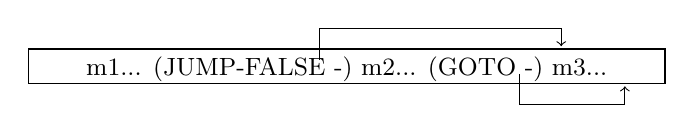
\begin{tikzpicture}
  \tikzstyle{every node}=[font=\small]

  \draw [semithick] (0em, 0em) rectangle (23em, 1.25em);
  \draw (11.5em, 1.33em) node[below]
        {\ic{m1... (JUMP-FALSE -) m2... (GOTO -) m3...}};

  \draw [->] (10.525em, 0.85em) -- (10.525em, 2em) --
             (19.25em, 2em) -- (19.25em, 1.35em);
  \draw [->] (17.75em, 0.35em) -- (17.75em, -0.75em) --
             (21.55em, -0.75em) -- (21.55em, -0.1em);

\end{tikzpicture}

\end{center}%
\caption{Линеаризованное ветвление.}%
\label{compilation/bytes/customize/lin-conditional/pic:subj}%
\end{figure}

С~использованием этих двух инструкций ветвление линеаризуется следующим
образом. (На~рисунке~\ref{compilation/bytes/customize/lin-conditional/pic:subj}
показано нагляднее.)

\indexC{ALTERNATIVE}
\begin{code:lisp}
(define (ALTERNATIVE m1 m2 m3)
  (append m1 (JUMP-FALSE (+ 1 (length m2))) m2 (GOTO (length m3)) m3) )
\end{code:lisp}

\ForLayout{display}{\endgroup}

Условие вычисляется, а затем проверяется \ic{JUMP-FALSE}. Если оно оказалось
истиной, то выполняются инструкции, непосредственно следующие за
\ic{JUMP-FALSE}, после чего \ic{GOTO} перебрасывает управление через
альтернативную ветку к~коду, следующему за ветвлением. Если~же условие ложно,
то управление просто передаётся альтернативной ветке. Как видим, для реализации
ветвления нам пришлось опуститься до уровня ассемблера. Кстати, обратите
внимание, что переходы выполняются относительно текущего значения счётчика
команд, а не~по абсолютным адресам.


\subsubsection{Линеаризация абстракций}%
\label{compilation/bytes/customize/sssect:lin-abstraction}

\indexR{линеаризация!абстракций}
\indexR{представление!замыканий!в машинном коде}
Последней из инструкций с~нетривиальной линеаризацией остаётся конструктор
замыканий. Проблема здесь в~том, как разместить код собственно функции и код,
замыкающий текущее окружение. Причём функцию не~надо сразу~же исполнять после
создания замыкания. Для реализации такого поведения снова используются переходы
(см.~рисунок~\ref{compilation/bytes/customize/lin-abstraction/pic:subj}). Вот
так создаются замыкания с~переменной арностью:

\indexC{NARY-CLOSURE}
\indexC{CREATE-CLOSURE}
\indexC{PACK-FRAME"!}
\begin{code:lisp}
(define (NARY-CLOSURE m+ arity)
  (define the-function
    (append (ARITY>=? (+ arity 1)) (PACK-FRAME! arity)
            (EXTEND-ENV) m+ (RETURN) ) )
  (append (CREATE-CLOSURE 1) (GOTO (length the-function))
          the-function ) )

(define (CREATE-CLOSURE offset)
  (list (lambda () (set! *val* (make-closure (list-tail *pc* offset)
                                             *env* )))) )
(define (PACK-FRAME! arity)
  (list (lambda () (listify! *val* arity))) )
\end{code:lisp}

\begin{figure}[t]\centering
% -*- coding: utf-8 -*-
% Линеаризованная абстракция
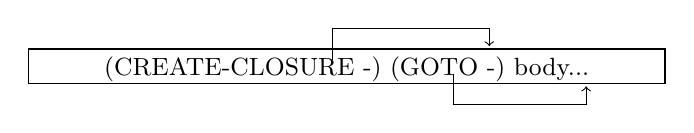
\begin{tikzpicture}
  \tikzstyle{every node}=[font=\small]

  \draw [semithick] (0em, 0em) rectangle (23em, 1.25em);
  \draw (11.5em, 1.33em) node[below]
        {\ic{(CREATE-CLOSURE -) (GOTO -) body...}};

  \draw [->] (11.00em, 0.85em) -- (11.00em, 2em) --
             (16.65em, 2em) -- (16.65em, 1.35em);
  \draw [->] (15.35em, 0.35em) -- (15.35em, -0.75em) --
             (20.15em, -0.75em) -- (20.15em, -0.1em);

\end{tikzpicture}
%
\caption{Линеаризованная абстракция.}%
\label{compilation/bytes/customize/lin-abstraction/pic:subj}%
\ForLayout{display}{\vskip-1.2\baselineskip}
\end{figure}

Новая машинная инструкция \ic{CREATE-CLOSURE} создаёт замыкание с~телом,
расположенным сразу~же за~\ic{GOTO}. Созданное замыкание кладётся в~регистр
\ic{*val*}, после чего мы перепрыгиваем через его код к~следующей инструкции
программы.


\subsection{Протокол вызова~функций}\label{compilation/bytes/ssect:call-proto}

\indexR{протокол вызова функций}
\indexR{функции!протокол вызова}
Вызовы функций выполняются с~помощью инструкций \ic{TR-REGULAR-CALL} и
\ic{REGULAR-CALL}, рассмотренных ранее.
\seePage[compilation/bytes/customize/sssect:lin-invocation]
Функция \ic{invoke} реализует протокол вызова функций:

\indexC{invoke}
\begin{code:lisp}
(define (invoke f)
  (cond ((closure? f)
         (stack-push *pc*)
         (set! *env* (closure-closed-environment f))
         (set! *pc* (closure-code f)) )
        ... ) )
\end{code:lisp}

Перед вызовом функции в~стек заталкивается адрес инструкции, следующей за
\ic{(FUNCTION-INVOKE)}. Затем извлекается сохранённое в~замыкании окружение и
устанавливается в~регистр \ic{*env*}. Наконец, в~регистр \ic{*pc*} заносится
адрес первой инструкции тела замыкания, что передаёт ему управление. Текущее
окружение здесь не~сохраняется: за управление ним отвечают непосредственно
\ic{REGULAR-CALL} и~\ic{TR-REGULAR-CALL}.

Следующей инструкцией, исполненной \ic{run}, будет первая инструкция вызванной
функции. Она проверяет арность и, в~случае успеха, расширяет текущее окружение
записью активации функции, в~тот момент уже находящейся в~регистре \ic{*val*}.
Теперь всё готово для исполнения тела функции. После его завершения в~регистре
\ic{*val*} будет находиться значение, которое требуется передать тому, кто
вызывал эту функцию. Возврат управления выполняет инструкция \ic{RETURN}. Ей
надо лишь восстановить значение \ic{*pc*}, ранее сохранённое в~стеке.

\indexC{RETURN}
\begin{code:lisp}
(define (RETURN)
  (list (lambda () (set! *pc* (stack-pop)))) )
\end{code:lisp}


\subsubsection{О~переходах}\label{compilation/bytes/sssect:jumps}

\indexR{позиционно-независимый код}
Если вы знакомы с~программированием на языке ассемблера, то наверняка обратили
внимание на то, что все переходы выполняются только вперёд по коду. Более того,
переходы являются относительными, равно как и адресация при создании замыканий.
Следовательно, получаемый машинный код никак не~зависит от своего фактического
расположения в~памяти, он \term{позиционно-независим}.


\section{Язык и целевая~машина}\label{compilation/sect:lang-and-target}

\indexR{виртуальная машина!архитектура}
Пришло время зафиксировать архитектуру целевой виртуальной машины, под которую
будут компилироваться программы, а также машинный язык, с~помощью которого ей
можно управлять. Как видно из
рисунка~\ref{compilation/lang-and-target/pic:subj}, машина имеет пять регистров:
\ic{*env*}, \ic{*val*}, \ic{*fun*}, \ic{*arg1*} и~\ic{*arg2*}, счётчик команд
\ic{*pc*}, а также стек.

\begin{figure}[tp]\begin{center}
% -*- coding: utf-8 -*-
% Архитектура целевой виртуальной машины
\begin{tikzpicture}
  \tikzstyle{every node}=[font=\footnotesize]

  \draw (0.00em,  0.00em) node[right] {\small\ic{*env*}};
  \draw (0.00em, -2.00em) node[right] {\small\ic{*val*}};
  \draw (0.00em, -4.00em) node[right] {\small\ic{*fun*}};
  \draw (0.00em, -6.00em) node[right] {\small\ic{*arg1*}};
  \draw (0.00em, -8.00em) node[right] {\small\ic{*arg2*}};

  \draw (0.00em,-10.00em) node[right] {\small\ic{*stack*}};
  \draw (0.00em,-11.25em) node[right] {\small\ic{*stack-index*}};

  \draw (0.00em,-13.25em) node[right] {\small\ic{*pc*}};

% *env*
  \draw [->] (3.00em, 0.00em) -- (5.75em, 0.00em);

  \draw             (6.15em, 0.00em) node[right] {\ic{next}};
  \draw [semithick] (6.00em, 0.50em) rectangle (9.00em, -3.50em);
  \draw             (6.00em,-0.50em) --  (9.00em, -0.50em);

  \filldraw  (8.50em, 0.00em) circle(1.0pt);
  \draw [->] (8.50em, 0.00em) -- (10.75em, 0.00em);

  \draw             (11.00em, 0.00em) node[right] {\ic{next}};
  \draw [semithick] (11.00em, 0.50em) rectangle (14.00em, -2.25em);
  \draw             (11.00em,-0.50em) --  (14.00em, -0.50em);

  \filldraw  (13.50em, 0.00em) circle(1.0pt);
  \draw [->] (13.50em, 0.00em) -- (15.75em, 0.00em);

  \draw             (16.00em, 0.00em) node[right] {\ic{next}};
  \draw [semithick] (16.00em, 0.50em) rectangle (19.00em, -5.00em);
  \draw             (16.00em,-0.50em) --  (19.00em, -0.50em);

  \filldraw  (18.50em, 0.00em) circle(1.0pt);
  \draw [->] (18.50em, 0.00em) -- (20.75em, 0.00em);
  
  \draw (20.75em, 0.10em) node[right] {\ii{nil}};

% *fun*
  \draw [->] (3.00em, -4.00em) -- (4.50em, -4.00em) --
             (4.50em, -5.75em) -- (22.75em, -5.75em);

  \draw [semithick] (23.00em, -5.00em) rectangle (29.00em, -6.50em);
  \draw [semithick] (26.25em, -5.00em) -- (26.25em, -6.50em);

  \draw (26.00em, -5.75em) node[left]  {\ic{code}};
  \draw (26.40em, -5.82em) node[right] {\ic{env}};
  \draw (29.25em, -7.10em) node[left] {\ii{замыкание}};
  
  \filldraw  (23.50em, -5.75em) circle(1.0pt);
  \draw [->] (23.50em, -5.75em) -- (23.50em, -19.00em) --
              (7.1em, -19.00em) --  (7.10em, -16.85em);

  \filldraw  (28.50em, -5.75em) circle(1.0pt);
  \draw [->] (28.50em, -5.75em) -- (28.50em, 1.50em) --
             (12.5em,   1.50em) -- (12.50em, 0.75em);
  
% *stack*
  \draw [semithick] (12.5em, -7.50em) rectangle (18.5em, -17.50em);
  \draw [loosely dashed, dash phase = 0.20em]
                    (12.5em, -10.50em) -- (18.5em, -10.50em);

  \draw [->] (4.00em, -10.00em) --  (7.50em, -10.00em) --
             (7.50em, -8.00em) -- (12.25em, -8.00em);
  \draw [->] (7.00em, -11.25em) -- (12.25em, -11.25em);

  \draw (15.5em,  -9.00em) node {\ii{используется}};
  \draw (15.5em, -13.75em) node {\ii{свободно}};

% *pc*
  \draw [->] (2.50em, -13.25em) -- (4.35em, -13.25em) -- (4.35em, -15.40em);

  \draw [semithick] (0.50em, -15.50em) rectangle (10.50em, -16.75em);
  \draw             (5.5em, -16.125em) node {\ic{... 34 250 41 4 34 ...}};

  \draw (0.25em, -17.35em) node[right] {\ii{байт-код}};

% *constants*
  \draw (29.75em, -9.90em) node[above] {\small\ic{*constants*}};
  \draw [semithick] (27.50em, -10.00em) rectangle (32.0em, -18.75em);
  \draw             (27.50em, -11.25em) -- (32.0em, -11.25em);
  \draw             (27.50em, -12.50em) -- (32.0em, -12.50em);
  \draw             (27.50em, -13.75em) -- (32.0em, -13.75em);
  \draw             (27.50em, -15.00em) -- (32.0em, -15.00em);
  \draw             (27.50em, -16.25em) -- (32.0em, -16.25em);
  \draw             (27.50em, -17.50em) -- (32.0em, -17.50em);

\end{tikzpicture}
\end{center}%
\caption{Архитектура целевой виртуальной машины.}%
\label{compilation/lang-and-target/pic:subj}%
\end{figure}

\indexC{FINISH}
Машинный язык состоит из тридцати четырёх инструкций. Все они собраны
в~таблице~\ref{compilation/lang-and-target/table:instructions}. Вдобавок к~ранее
рассмотренным, мы ввели инструкцию \ic{FINISH}, которая завершает исполнение
программы (фактически, выходит из функции \ic{run}) и возвращает управление
тому, кто запустил нашу виртуальную машину.

\indexR{инструкции!простые и составные}
Все двадцать пять инструкций"=генераторов промежуточного языка можно разделить
на две группы: простые инструкции и составные. Простые инструкции имеют
непосредственные аналоги в~машинном языке, они отмечены звёздочками
в~таблице~\ref{compilation/lang-and-target/table:instructions}.
В~противоположность им, шестнадцать составных инструкций промежуточного языка
определяются через оставшиеся двадцать пять машинных. Мы могли~бы разбивать
инструкции на машинные команды более агрессивно, например, разделив
\ic{CHECKED-GLOBAL-REF} на \ic{GLOBAL-REF} и отдельную инструкцию, проверяющую,
действительно~ли в~\ic{*val*} лежит значение инициализированной переменной, но
это~бы замедлило интерпретацию. Так что скорее наоборот, некоторые инструкции
имеет смысл объединить, например: \ic{POP-ARG2} используется только
в~\ic{CALL3}, причём за \ic{POP-ARG2} всегда следует \ic{POP-ARG1}, поэтому 
данную пару вполне можно превратить в~отдельную инструкцию.

\begin{table}[!htb]%
\indexR{виртуальная машина!язык}%
\indexR{язык!машинный}%
\def\I{\ii{i}} \def\J{\ii{j}} \def\V{\ii{v}}
\def\star{\textsubscript{\ic{*}}}
\def\P{\normalfont\:+\:1}
\def\botstrut{\rule[-0.6em]{0pt}{\baselineskip}}
\def\topstrut{\rule[1.25em]{0pt}{\baselineskip}}
\setlength{\tabcolsep}{0.5em}
\begin{center}\begin{tabular}{|l|l|}
\hline\topstrut%
\ic{(SHALLOW-ARGUMENT-REF \J)}\star  & \ic{(PREDEFINED \I)}\star              \\
\ic{(DEEP-ARGUMENT-REF \I\ \J)}\star & \ic{(SET-SHALLOW-ARGUMENT! \J)}        \\
\ic{(SET-DEEP-ARGUMENT! \I\ \J)}     & \ic{(GLOBAL-REF \I)}\star              \\
\ic{(CHECKED-GLOBAL-REF \I)}\star    & \ic{(SET-GLOBAL! \I)}                  \\
\ic{(CONSTANT \V)}\star              & \ic{(JUMP-FALSE \ii{смещение})}        \\
\ic{(GOTO \ii{смещение})}            & \ic{(EXTEND-ENV)}                      \\
\ic{(UNLINK-ENV)}                    & \ic{(CALL0 \ii{адрес})}\star           \\
\ic{(INVOKE1 \ii{адрес})}            & \ic{(PUSH-VALUE)}                      \\
\ic{(INVOKE2 \ii{адрес})}            & \ic{(POP-ARG1)}                        \\
\ic{(INVOKE3 \ii{адрес})}            & \ic{(POP-ARG2)}                        \\
\ic{(CREATE-CLOSURE \ii{смещение})}  & \ic{(ARITY=? \ii{арность}\P)}          \\
\ic{(RETURN)}                        & \ic{(ARITY>=? \ii{арность}\P)}         \\
\ic{(PACK-FRAME! \ii{арность})}      & \ic{(POP-FUNCTION)}                    \\
\ic{(FUNCTION-INVOKE)}               & \ic{(PRESERVE-ENV)}                    \\
\ic{(RESTORE-ENV)}                   & \ic{(POP-FRAME! \ii{индекс})}          \\
\ic{(POP-CONS-FRAME! \ii{арность})}  & \ic{(ALLOCATE-FRAME \ii{размер})}\star \\
\ic{(ALLOCATE-DOTTED-FRAME \ii{арность})}\star & \ic{(FINISH)}\botstrut       \\
\hline
\end{tabular}\end{center}%
\caption{Символьная форма машинных инструкций.}%
\label{compilation/lang-and-target/table:instructions}%
\end{table}

Тривиальной части составных инструкций мы не~касались, но их определения
на машинном языке всё~же стоит привести. Они собраны ниже, без каких-либо
пояснений. Некоторые из~машинных инструкций из
таблицы~\ref{compilation/lang-and-target/table:instructions} тоже не~были
определены, ими мы займёмся чуть~позже.

\indexC{DEEP-ARGUMENT-SET"!}
\indexC{GLOBAL-SET"!}
\indexC{SEQUENCE}
\indexC{TR-FIX-LET}
\indexC{FIX-LET}
\indexC*{CALL0}{CALL\protect\ii{n}}
\indexC{FIX-CLOSURE}
\indexC{TR-REGULAR-CALL}
\indexC{STORE-ARGUMENT}
\indexC{CONS-ARGUMENT}
\begin{code:lisp}
(define (DEEP-ARGUMENT-SET! i j m)
  (append m (SET-DEEP-ARGUMENT! i j)) )

(define (GLOBAL-SET! i m)
  (append m (SET-GLOBAL! i)) )

(define (SEQUENCE m m+)
  (append m m+) )

(define (TR-FIX-LET m* m+)
  (append m* (EXTEND-ENV) m+) )

(define (FIX-LET m* m+)
  (append m* (EXTEND-ENV)
          m+ (UNLINK-ENV) ) )

(define (CALL1 address m1)
  (append m1 (INVOKE1 address)) )

(define (CALL2 address m1 m2)
  (append m1 (PUSH-VALUE)
          m2 (POP-ARG1)
          (INVOKE2 address) ) )

(define (CALL3 address m1 m2 m3)
  (append m1 (PUSH-VALUE)
          m2 (PUSH-VALUE)
          m3 (POP-ARG2) (POP-ARG1)
          (INVOKE3 address) ) )

(define (FIX-CLOSURE m+ arity)
  (define the-function
    (append (ARITY=? (+ arity 1))
            (EXTEND-ENV) m+
            (RETURN) ) )
  (append (CREATE-CLOSURE 1)
          (GOTO (length the-function))
          the-function ) )

(define (TR-REGULAR-CALL m m*)
  (append m (PUSH-VALUE)
          m* (POP-FUNCTION)
          (FUNCTION-INVOKE) ) )

(define (STORE-ARGUMENT m m* index)
  (append m (PUSH-VALUE)
          m* (POP-FRAME! index) ) )

(define (CONS-ARGUMENT m m* arity)
  (append m (PUSH-VALUE)
          m* (POP-CONS-FRAME! arity) ) )
\end{code:lisp}

\phantomlabel{compilation/lang-and-target/par:slowpoke}
\indexR{однопроходная компиляция}
\indexR{компиляция!однопроходная}
\indexR{линеаризация!кодогенерации}
Вызовы \ic{append}, коими кишат наши определения, довольно ощутимо замедляют
кодогенерацию. Хорошим решением будет собирать машинные инструкции
в~последовательность за один проход. Именно так мы и поступим при разработке
компилятора в~Си. \seePage[cc/gen/ssect:exprs] Для реализации подобного подхода
потребуется вдобавок к~линеаризации самого машинного кода также линеаризовать и
его генераторы. Например, \ic{CALL2} должна работать в~такой последовательности:

\begin{enumerate}
  \item сгенерировать и вывести код~\ic{m1};
  \item вывести код \ic{(PUSH-VALUE)};
  \item сгенерировать и вывести код~\ic{m2};
  \item вывести код \ic{(POP-ARG1)};
  \item вывести код \ic{(INVOKE2~\ii{адрес})}.
\end{enumerate}

\indexCS{GOTO}{правки задним числом}
\indexCS{JUMP-FALSE}{правки задним числом}
\indexE{backpatching}
\phantomlabel{compilation/lang-and-target/par:backtracking}
Подобные изменения легко сделать всюду, кроме \ic{GOTO} и \ic{JUMP-FALSE}, так
как теперь не~получится заранее вычислить смещения при генерации кода для
\ic{ALTERNATIVE}, \ic{FIX-CLOSURE} и~\ic{NARY-CLOSURE}. Это затруднение
можно решить правкой смещений задним числом (такой приём называется
\term{backpatching}). Например, для \ic{FIX-CLOSURE} следует делать~так:

\begin{enumerate}
  \item вывести инструкцию \ic{CREATE-CLOSURE};
  
  \item вывести инструкцию \ic{GOTO}, но без смещения, запомнив при этом
        текущее состояние счётчика команд;
  
  \item сгенерировать и вывести код тела функции;
  
  \item зная текущее значение счётчика команд и помня сохранённое ранее,
        вычислить величину смещения для \ic{GOTO};
  
  \item записать это число на зарезервированное\footnote{Вот здесь могут
        возникнуть некоторые проблемы, потому что смещение может оказаться
        как меньшим~256, так и превышать это значение, то~есть занимать
        один или два байта. Это может оказаться причиной определённых
        потерь производительности.} внутри \ic{GOTO} место.
\end{enumerate}

В~результате получится более аккуратная и эффективная процедура генерации кода,
чем есть сейчас, но пока мы всё~же оставим текущий вариант из"~за его простоты.


\subsection{Дизассемблирование}%
\label{compilation/lang-and-target/ssect:disassembly}

В~начале этой главы \seePage[compilation/par:disasm] была показана промежуточная
форма следующей небольшой программки:

\indexC{fact}
\begin{code:lisp}
((lambda (fact) (fact 5 fact (lambda (x) x)))
 (lambda (n f k) (if (= n 0) (k 1)
                     (f (- n 1) f (lambda (r) (k (* n r)))) )) )
\end{code:lisp}

Теперь, наконец, мы сможем увидеть, как она выглядит на настоящем машинном
языке. Сложно не~заметить сходство
таблицы~\ref{compilation/lang-and-target/disassembly/table:subj} с~ассемблерным
листингом.

\begin{table}[pt]\setlength{\tabcolsep}{1.5em}%
\begin{center}\begin{tabular}{l|@{\extracolsep{1.25em}}l}
\ic{(CREATE-CLOSURE 2)}          &   \ic{(INVOKE2 \#<*>)}            \\
\ic{(GOTO 82)}                   &   \ic{(PUSH-VALUE)}               \\
\ic{(ARITY=? 4)}                 &   \ic{(ALLOCATE-FRAME 1)}         \\
\ic{(EXTEND-ENV)}                &   \ic{(POP-FRAME! 0)}             \\
\ic{(SHALLOW-ARGUMENT-REF 0)}    &   \ic{(POP-FUNCTION)}             \\
\ic{(PUSH-VALUE)}                &   \ic{(FUNCTION-INVOKE)}          \\
\ic{(CONSTANT 0)}                &   \ic{(RETURN)}                   \\
\ic{(POP-ARG1)}                  &   \ic{(PUSH-VALUE)}               \\
\ic{(INVOKE2 \#<=>)}             &   \ic{(ALLOCATE-FRAME 3)}         \\
\ic{(JUMP-FALSE 13)}             &   \ic{(POP-FRAME! 2)}             \\
\ic{(SHALLOW-ARGUMENT-REF 2)}    &   \ic{(POP-FRAME! 1)}             \\
\ic{(PUSH-VALUE)}                &   \ic{(POP-FRAME! 0)}             \\
\ic{(CONSTANT 1)}                &   \ic{(POP-FUNCTION)}             \\
\ic{(PUSH-VALUE)}                &   \ic{(FUNCTION-INVOKE)}          \\
\ic{(ALLOCATE-FRAME 1)}          &   \ic{(RETURN)}                   \\
\ic{(POP-FRAME! 0)}              &   \ic{(PUSH-VALUE)}               \\
\ic{(POP-FUNCTION)}              &   \ic{(ALLOCATE-FRAME 1)}         \\
\ic{(FUNCTION-INVOKE)}           &   \ic{(POP-FRAME! 0)}             \\
\ic{(GOTO 54)}                   &   \ic{(EXTEND-ENV)}               \\
\ic{(SHALLOW-ARGUMENT-REF 1)}    &   \ic{(SHALLOW-ARGUMENT-REF 0)}   \\
\ic{(PUSH-VALUE)}                &   \ic{(PUSH-VALUE)}               \\
\ic{(SHALLOW-ARGUMENT-REF 0)}    &   \ic{(CONSTANT 5)}               \\
\ic{(PUSH-VALUE)}                &   \ic{(PUSH-VALUE)}               \\
\ic{(CONSTANT 1)}                &   \ic{(SHALLOW-ARGUMENT-REF 0)}   \\
\ic{(POP-ARG1)}                  &   \ic{(PUSH-VALUE)}               \\
\ic{(INVOKE2 \#<->)}             &   \ic{(CREATE-CLOSURE 2)}         \\
\ic{(PUSH-VALUE)}                &   \ic{(GOTO 6)}                   \\
\ic{(SHALLOW-ARGUMENT-REF 1)}    &   \ic{(ARITY=? 2)}                \\
\ic{(PUSH-VALUE)}                &   \ic{(EXTEND-ENV)}               \\
\ic{(CREATE-CLOSURE 2)}          &   \ic{(SHALLOW-ARGUMENT-REF 0)}   \\
\ic{(GOTO 24)}                   &   \ic{(RETURN)}                   \\
\ic{(ARITY=? 2)}                 &   \ic{(PUSH-VALUE)}               \\
\ic{(EXTEND-ENV)}                &   \ic{(ALLOCATE-FRAME 3)}         \\
\ic{(DEEP-ARGUMENT-REF 1 2)}     &   \ic{(POP-FRAME! 2)}             \\
\ic{(PUSH-VALUE)}                &   \ic{(POP-FRAME! 1)}             \\
\ic{(DEEP-ARGUMENT-REF 1 0)}     &   \ic{(POP-FRAME! 0)}             \\
\ic{(PUSH-VALUE)}                &   \ic{(POP-FUNCTION)}             \\
\ic{(SHALLOW-ARGUMENT-REF 0)}    &   \ic{(FUNCTION-INVOKE)}          \\
\ic{(POP-ARG1)}                  &   \ic{(RETURN)}
\end{tabular}\end{center}%
\caption{Результат компиляции.}%
\label{compilation/lang-and-target/disassembly/table:subj}%
\end{table}


\section{Кодирование инструкций}\label{compilation/sect:coding}

\indexR{байт-код}
Почти на каждой странице этой главы упоминаются байты, но до сих пор мы
не~видели ни~одного из них живьём. К~счастью, чтобы они появились, достаточно
лишь по-другому понимать инструкции
таблицы~\ref{compilation/lang-and-target/table:instructions}: теперь это
не~непосредственно исполнимые команды, а генераторы последовательностей байтов
"--- исходного кода для другой, более быстрой функции \ic{run}. Сейчас мы
сконцентрируемся именно на этом аспекте байт-кода: его компактности и~скорости
интерпретации.

\indexR{макросы!применения}
Байт-кодирование требует особой осторожности: за каждой инструкцией должно быть
закреплено уникальное число, по которому определяется её поведение внутри
\ic{run}, длина операндов этой инструкции, а также многое другое. Поэтому, чтобы
в~процессе ничего не~напутать, инструкции будут определяться с~помощью макроса
\ic{define-instruction}. При этом предполагается, что все определения машинных
инструкций на самом деле обёрнуты в~макрос \ic{define-instruction-set}, который
кроме собственно формы \ic{define-instruction} определяет также несколько
вспомогательных функций.

\indexC{define-instruction-set}
\indexC{run}
\indexC{instruction-size}
\indexC{instruction-decode}
\indexC{run-clause}
\indexC{size-clause}
\begin{code:lisp}
(define-syntax define-instruction-set
  (syntax-rules (define-instruction)
    ((define-instruction-set
       (define-instruction (name . args) n . body) ... )
     (begin
       (define (run)
         (let ((instruction (fetch-byte)))
           (case instruction
             ((n) (run-clause args body)) ... ) )
         (run) )

       (define (instruction-size code pc)
         (let ((instruction (vector-ref code pc)))
           (case instruction
             ((n) (size-clause args)) ... ) ) )

       (define (instruction-decode code pc)
         (define (fetch-byte)
           (let ((byte (vector-ref code pc)))
             (set! pc (+ pc 1))
             byte ) )
         (let-syntax
             ((decode-clause
               (syntax-rules ()
                 ((decode-clause iname ())
                  '(iname) )
                 ((decode-clause iname (a))
                  (let ((a (fetch-byte)))
                    (list 'iname a) ) )
                 ((decode-clause iname (a b))
                  (let* ((a (fetch-byte))
                         (b (fetch-byte)) )
                    (list 'iname a b) ) ) ) ))
           (let ((instruction (fetch-byte)))
             (case instruction
               ((n) (decode-clause name args)) ... ) ) ) ) ) ) ) )

(define-syntax run-clause
  (syntax-rules ()
    ((run-clause () body)
     (begin . body) )
    ((run-clause (a) body)
     (let ((a (fetch-byte)))
       . body ) )
    ((run-clause (a b) body)
     (let* ((a (fetch-byte))
            (b (fetch-byte)) )
       . body ) ) ) )

(define-syntax size-clause
  (syntax-rules ()
    ((size-clause ())    1)
    ((size-clause (a))   2)
    ((size-clause (a b)) 3) ) )
\end{code:lisp}

Макрос \ic{define-instruction} одновременно определяет сразу три функции:
функцию \ic{run}, исполняющую байт-коды; функцию \ic{instruction-size},
возвращающую размер инструкций; и~функцию \ic{instruction-decode},
переводящую байт-код обратно в~символьную форму. Очевидно,
\ic{instruction-decode}, будет весьма полезной при отладке. Рассмотрим пример:

\begin{code:lisp}
(define-instruction (SHALLOW-ARGUMENT-REF j) 5
  (set! *val* (activation-frame-argument *env* j)) )
\end{code:lisp}

Эта форма добавляет в~определение \ic{run} обработку инструкции, кодируемой
числом~\ic{5}:

\begin{code:lisp}
(define (run)
  (let ((instruction (fetch-byte)))
    (case instruction
      ...
      ((5) (let ((j (fetch-byte)))
             (set! *val* (activation-frame-argument *env* j)) ))
      ... ) )
  (run) )
\end{code:lisp}

\indexC{fetch-byte}
Функция \ic{fetch-byte} используется для извлечения операндов инструкции из
потока байтов. Она очень просто определяется и имеет один побочный эффект: сдвиг
\ic{*pc*} на одну позицию вперёд.

\begin{code:lisp}
(define (fetch-byte)
  (let ((byte (vector-ref *code* *pc*)))
    (set! *pc* (+ 1 *pc*))
    byte ) )
\end{code:lisp}

\indexR{счётчик команд}
Также \ic{fetch-byte} используется функцией \ic{run} для считывания следующей
инструкции. Кстати, обратите внимание, что счётчик команд всегда указывает на
\emph{следующую} инструкцию, а не~на текущую исполняемую. Точно такое~же решение
применяется и во~многих настоящих процессорах.

\indexCS{case}{таблица переходов}
Для достижения действительно высокой скорости интерпретации (другими словами,
чтобы получить быструю \ic{run}) следует уделить особое внимание используемой
здесь форме \ic{case}. Благодаря тому, что дискриминант \ic{case} может быть
только числом от~0 до~255, становится возможным реализовать \ic{case} через
таблицу переходов, что позволит выполнять выбор нужной ветви за постоянное
время. Если~же \ic{case} раскрывается в~цепочку \ic{(if (eqv?~...) ...)}, то
выбор выполняется за линейное время "--- прощай, производительность! Лишь
некоторые из компиляторов Лиспа умеют выполнять такую оптимизацию автоматически
(среди них Sqil~\cite{sen91} и Bigloo~\cite{ser93}).

\ic{define-instruction} также принимает участие в~определении функции
\ic{instruction-size}: туда она добавляет информацию о~том, что инструкция
\ic{SHALLOW-ARGUMENT-REF} занимает два байта. Аналогично, здесь \ic{case} можно
заменить вектором, хранящим те~же самые числа.

\begin{code:lisp}
(define (instruction-size code pc)
  (let ((instruction (vector-ref code pc)))
    (case instruction
      ...
      ((5) 2)
      ... ) ) )
\end{code:lisp}

\indexC{fetch-byte}
Наконец, \ic{define-instruction} добавляет в~\ic{instruction-decode},
ветку для обработки инструкции \ic{SHALLOW-ARGUMENT-REF}. Функция
\ic{instruction-decode} использует свою личную реализацию \ic{fetch-byte},
чтобы вести себя подобно \ic{run}, но не~влиять на глобальный счётчик команд.

\begin{code:lisp}
(define (instruction-decode code pc)
  (define (fetch-byte)
    (let ((byte (vector-ref code pc)))
      (set! pc (+ pc 1))
      byte ) )
  (let ((instruction (vector-ref code pc)))
    (case instruction
      ...
      ((5) (let ((j (fetch-byte)))
             (list 'SHALLOW-ARGUMENT-REF j) ))
      ... ) ) )
\end{code:lisp}


\section{Инструкции}\label{compilation/sect:instructions}

\indexR{инструкции!распределение арности}
\indexR{арность}
\indexR{байт-код!использование излишков}
\indexR{специализация!машинных инструкций}
Всего существует 256 возможных кодов инструкций, мы~же используем только 34 из
них. Настало время задействовать эти резервы; вспомните, как мы предлагали
объединять инструкции, которые часто используются вместе. Кроме того очевиден
\cite{cha80} тот факт, что большинство функций имеет небольшое число аргументов.
Действительно, достаточно лишь посмотреть на функции, использованные в~данной
книге. Их анализ показывает следующие результаты: лишь 16~функций имеют
переменную арность; распределение арности остальных~1988 приведено
в~таблице~\ref{compilation/instructions/table:probs}.

\begin{table}[!ht]\renewcommand*{\arraystretch}{1.15}
\begin{center}\begin{tabular}{lccccccccc}
\hline%
арность        &  0 &  1 &  2 &  3 &  4 &  5 &  6 &  7 &   8 \\
\hline%
доля,~\%       & 35 & 30 & 18 &  9 &  4 &  1 &  0 &  0 &   0 \\
накопление,~\% & 35 & 66 & 84 & 93 & 97 & 99 & 99 & 99 & 100
\end{tabular}\end{center}%
\caption{Распределение функций по количеству аргументов.}%
\label{compilation/instructions/table:probs}%
\end{table}

Как видим, подавляющее большинство функций имеет не~более четырёх аргументов.
При обобщении этих результатов следует учесть, что настолько большие числа для
нулевой арности получены в~основном благодаря шестой главе. Итого, однозначно
имеет смысл оптимизировать вызовы функций, принимающих менее четырёх аргументов.
Этим мы и займёмся, используя избыточные коды инструкций для создания
специализированных вариантов.


\subsection{Локальные переменные}\label{compilation/instructions/ssect:locals}

\indexC{LAMBDA-PARAMETERS-LIMIT}
\indexC{check-byte}
\indexR{функции!максимальное количество аргументов}
Пожалуй, давайте начнём с~\ic{SHALLOW-ARGUMENT-REF}. Эта инструкция имеет один
операнд:~$j$, а её действие заключается в~том, что регистр \ic{*val*} получает
значение $j$"~й локальной переменной текущей записи активации, хранящейся
в~регистре \ic{*env*}. Здесь можно ввести специализации для случаев $j = 0, 1,
2, 3$, сделав каждый из них отдельной инструкцией со~своим кодом. Также для
простоты можно ввести ограничение\footnote{В~{\CommonLisp} даже есть специальная
константа \ic{LAMBDA-PARAMETERS-LIMIT}, хранящая максимально возможно количество
аргументов функции. По стандарту оно не~может быть меньше~50. Стандарт Scheme
ничего не~говорит о~подобных ограничениях, но его молчание можно толковать
по-разному.\par Как~бы то ни~было, вопрос представления чисел интересен сам по
себе. В~большинстве систем, поддерживающих длинную арифметику, максимально
представимое число немного меньше, чем $256^{2^{32}}$. (Чуть-чуть не~хватило до
бесконечности.) Хитрость в~том, что перед длинным числом записывается его длина
в~байтах. Аналогичное решение можно применить и здесь.} в~256~аргументов
функции "--- это позволит всегда кодировать индекс аргумента одним"=единственным
байтом. Функция \ic{check-byte}\footnote{В~последующих определениях мы не~будем
упоминать \ic{check-byte} ради краткости.} убеждается в~соблюдении этого
ограничения. Итак, вот определение \ic{SHALLOW-ARGUMENT-REF}. Эта инструкция
является генератором байт-кодов "--- она возвращает список\footnote{Да"~да,
\ic{list}, \ic{append}, неэффективно,
страница~\pageref{compilation/lang-and-target/par:slowpoke}. Извините.} байтов,
соответствующих кодируемой инструкции. Этот список состоит из одного или двух
байтов, в~зависимости от операнда.

\indexCS{SHALLOW-ARGUMENT-REF}{специализация}
\indexC{check-byte}
\begin{code:lisp}
(define (SHALLOW-ARGUMENT-REF j)
  (check-byte j)
  (case j
    ((0 1 2 3) (list (+ 1 j)))
    (else      (list 5 j)) ) )

(define (check-byte j)
  (unless (<= 0 j 255)
    (static-wrong "Cannot pack a number within a byte" j) ) )
\end{code:lisp}

А~вот определения собственно пяти\footnote{Инструкции с~кодом~\ic{0}
не~существует "--- бедный ноль и без того особенный.} специализаций:

\begin{code:lisp}
(define-instruction (SHALLOW-ARGUMENT-REF0) 1
  (set! *val* (activation-frame-argument *env* 0)) )
(define-instruction (SHALLOW-ARGUMENT-REF1) 2
  (set! *val* (activation-frame-argument *env* 1)) )
(define-instruction (SHALLOW-ARGUMENT-REF2) 3
  (set! *val* (activation-frame-argument *env* 2)) )
(define-instruction (SHALLOW-ARGUMENT-REF3) 4
  (set! *val* (activation-frame-argument *env* 3)) )
(define-instruction (SHALLOW-ARGUMENT-REF j) 5
  (set! *val* (activation-frame-argument *env* j)) )
\end{code:lisp}

\ic{SET-SHALLOW-ARGUMENT!} тоже работает с~локальными переменными, так что
определяется аналогично. (Пропущенные здесь специализации легко определить
самостоятельно.)

\indexCS{SET-SHALLOW-ARGUMENT"!}{специализация}
\begin{code:lisp}
(define (SET-SHALLOW-ARGUMENT! j)
  (case j
    ((0 1 2 3) (list (+ 21 j)))
    (else      (list 25 j)) ) )

(define-instruction (SET-SHALLOW-ARGUMENT!2) 23
  (set-activation-frame-argument! *env* 2 *val*) )
(define-instruction (SET-SHALLOW-ARGUMENT! j) 25
  (set-activation-frame-argument! *env* j *val*) )
\end{code:lisp}

\indexCS{DEEP-ARGUMENT-REF}{специализация}
\indexCS{SET-DEEP-ARGUMENT"!}{специализация}
Что касается свободных переменных, то мы предполагаем,\footnote*{Вообще"~то это
не~совсем верное предположение, ведь мы только что убедились в~том, что $j$ чаще
всего оказывается меньше четырёх. Но так как свободные переменные используются
значительно реже локальных и глобальных, то можно не~особо спешить с~ускорением
доступа к~ним.} что их индексы равновероятны, поэтому для них специализаций
не~будет:

\begin{code:lisp}
(define (DEEP-ARGUMENT-REF i j) (list 6 i j))
(define (SET-DEEP-ARGUMENT! i j) (list 26 i j))

(define-instruction (DEEP-ARGUMENT-REF i j) 6
  (set! *val* (deep-fetch *env* i j)) )
(define-instruction (SET-DEEP-ARGUMENT! i j) 26
  (deep-update! *env* i j *val*) )
\end{code:lisp}


\subsection{Глобальные переменные}\label{compilation/instructions/ssect:globals}

\indexR{глобальные переменные}
\indexR{переменные!глобальные}
\indexR{представление!глобальных переменных}
\indexR{глобальное окружение!машинная реализация}
\indexR{окружение!глобальное}
Про распределение глобальных изменяемых переменных, определяемых пользователем,
виртуальная машина ничего знать не~может в~принципе, так что они тоже будут
кодироваться без специализаций. Для простоты предположим, что глобальных
переменных может быть не~более~256, что позволит закодировать их адрес одним
байтом. Таким образом, имеем следующее:

\indexCS{GLOBAL-REF}{специализация}
\indexCS{CHECKED-GLOBAL-REF}{специализация}
\indexCS{SET-GLOBAL"!}{специализация}
\begin{code:lisp}
(define (GLOBAL-REF i) (list 7 i))
(define (CHECKED-GLOBAL-REF i) (list 8 i))
(define (SET-GLOBAL! i) (list 27 i))

(define-instruction (GLOBAL-REF i) 7
  (set! *val* (global-fetch i)) )

(define-instruction (CHECKED-GLOBAL-REF i) 8
  (set! *val* (global-fetch i))
  (when (eq? *val* undefined-value)
    (signal-exception #t (list "Uninitialized global variable" i)) ) )

(define-instruction (SET-GLOBAL! i) 27
  (global-update! i *val*) )
\end{code:lisp}

Случай предопределённых неизменяемых переменных более интересен, так как доступ
к~наиболее часто используемым из них можно немного ускорить. В~список таких
переменных включены \ic{t}, \ic{f}, \ic{nil}, \ic{cons}, \ic{car} и некоторые
другие.

\ForLayout{display}{\begingroup
\lstset{aboveskip=\smallskipamount, belowskip=\smallskipamount}}

\indexCS{PREDEFINED}{специализация}
\begin{code:lisp}
(define (PREDEFINED i)
  (check-byte i)
  (case i
    ;; \ic{0}${}={}$\ic{\#t}, \ic{1}${}={}$\ic{\#f}, \ic{2}${}={}$\ic{()},%
    {} \ic{3}${}={}$\ic{cons}, \ic{4}${}={}$\ic{car},
    ;; \ic{5}${}={}$\ic{cdr}, \ic{6}${}={}$\ic{pair?},%
    {} \ic{7}${}={}$\ic{symbol?}, \ic{8}${}={}$\ic{eq?}
    ((0 1 2 3 4 5 6 7 8) (list (+ 10 i)))
    (else                (list 19 i)) ) )

(define-instruction (PREDEFINED0) 10    ; \ic{\#t}
  (set! *val* #t) )
(define-instruction (PREDEFINED i) 19
  (set! *val* (predefined-fetch i)) )
\end{code:lisp}

\indexE{constants@\protect\ic{*constants*}}
\indexR{регистры!constants@\protect\ic{*constants*}}
\indexR{цитаты}
Раз уж некоторые константы трактуются по-особому, то давайте так~же поступим и
с~цитатами. Предположим, в~машине имеется регистр \ic{*constants*}, содержащий
вектор всех используемых в~программе цитат, тогда доступ к~ним можно получить
с~помощью функции \ic{quotation-fetch}:

\indexC{quotation-fetch}
\begin{code:lisp}
(define (quotation-fetch i)
  (vector-ref *constants* i) )
\end{code:lisp}

Комбинатор \ic{CONSTANT} собирает все цитаты в~переменной \ic{*quotations*}
во~время компиляции. Перед исполнением программы все используемые цитаты
загружаются в~регистр \ic{*constants*}. Цитаты не~равновероятны: некоторые из
них используются чаще других, поэтому им будут выданы собственные инструкции.
Часть из них по очевидным причинам совпадает с~предопределёнными константами
вроде \ic{PREDEFINED0}. Наконец, мы предположим, что цитировать напрямую
в~машинном коде можно только целые числа от~0 до~255, остальные будут на общих
правах размещаться в~\ic{*constants*}.\footnote*{Это досадно, но где"~то~же
должна проходить граница между обычными числами и длинными.}

\indexCS{CONSTANT}{специализация}
\indexC{SHORT-NUMBER}
\indexC{EXPLICIT-CONSTANT}
\begin{code:lisp}
(define (CONSTANT value)
  (cond ((eq? value #t)    (list 10))
        ((eq? value #f)    (list 11))
        ((eq? value '())   (list 12))
        ((equal? value -1) (list 80))
        ((equal? value 0)  (list 81))
        ((equal? value 1)  (list 82))
        ((equal? value 2)  (list 83))
        ((equal? value 3)  (list 84))
        ((and (integer? value)   ; непосредственное значение
              (<= 0 value 255) )
         (list 79 value) )
        (else (EXPLICIT-CONSTANT value)) ) )

(define (EXPLICIT-CONSTANT value)
  (set! *quotations* (append *quotations* (list value)))
  (list 9 (- (length *quotations*) 1)) )

(define-instruction (CONSTANT-1) 80
  (set! *val* -1) )
(define-instruction (CONSTANT0) 81
  (set! *val* 0) )
(define-instruction (SHORT-NUMBER value) 79
  (set! *val* value) )
\end{code:lisp}

\ForLayout{display}{\endgroup}

\subsection{Переходы}\label{compilation/instruction/ssect:jumps}

\indexR{переходы (jumps)!произвольная дальность}
Если вы думаете, что расставленные то~тут, то~там ограничения чересчур суровы,
тогда этот раздел для вас. Очевидно, что не~стоит ограничивать \ic{GOTO} или
\ic{JUMP-FORWARD} прыжками максимум на 256~байтов вперёд,\footnote*{На~некоторых
старых машинах, основанных на процессоре i8086, такое ограничение действительно
существовало.} так как код без проблем может превысить эти размеры. Поэтому мы
будем различать случаи, когда длина прыжка записывается одним или двумя байтами.
Введём две отдельные инструкции\footnote{Очевидно, что подобное разделение на
\ic{SHORT}- и \ic{LONG}-версию может быть применено, например, к~\ic{GLOBAL-REF}
с~компанией, чтобы количество изменяемых глобальных переменных больше не~было
ограничено 256"~ю.}: \ic{SHORT-GOTO} и \ic{LONG-GOTO}. Думаем, этого будет
достаточно на время; наш компилятор пока не~метит в~олимпийские чемпионы, чтобы
прыгать дальше 64~килобайт.

\indexCS{GOTO}{специализация}
\indexCS{JUMP-FALSE}{специализация}
\begin{code:lisp}
(define (GOTO offset)
  (cond ((< offset 256) (list 30 offset))
        ((< offset 65536)
         (let ((offset1 (modulo offset 256))
               (offset2 (quotient offset 256)) )
           (list 28 offset1 offset2) ) )
        (else (static-wrong "Too long jump" offset)) ) )

(define (JUMP-FALSE offset)
  (cond ((< offset 256) (list 31 offset))
        ((< offset 65536)
         (let ((offset1 (modulo offset 256))
               (offset2 (quotient offset 256)) )
           (list 29 offset1 offset2) ) )
        (else (static-wrong "Too long jump" offset)) ) )

(define-instruction (SHORT-GOTO offset) 30
  (set! *pc* (+ *pc* offset)) )

(define-instruction (SHORT-JUMP-FALSE offset) 31
  (if (not *val*) (set! *pc* (+ *pc* offset))) )

(define-instruction (LONG-GOTO offset1 offset2) 28
  (let ((offset (+ offset1 (* 256 offset2))))
    (set! *pc* (+ *pc* offset)) ) )
\end{code:lisp}


\subsection{Вызовы функций}\label{compilation/instruction/ssect:invocations}

Для начала разберёмся с~обычными вызовами, а потом перейдём ко~встраиваемым.
Наблюдение о~преимущественно небольшой арности используемых функций будет
полезным и~здесь. Выделив ещё немного байт-кодов, мы можем специализировать
создание записей активаций для малого числа аргументов:

\indexCS{ALLOCATE-FRAME}{специализация}
\begin{code:lisp}
(define (ALLOCATE-FRAME size)
  (case size
    ((0 1 2 3 4) (list (+ 50 size)))
    (else        (list 55 (+ size 1))) ) )

(define-instruction (ALLOCATE-FRAME1) 50
  (set! *val* (allocate-activation-frame 1)) )
(define-instruction (ALLOCATE-FRAME size+1) 55
  (set! *val* (allocate-activation-frame size+1)) )
\end{code:lisp}

Раскладывание значений аргументов по записям тоже можно улучшить для небольших
арностей:

\indexCS{POP-FRAME"!}{специализация}
\begin{code:lisp}
(define (POP-FRAME! index)
  (case index
    ((0 1 2 3) (list (+ 60 index)))
    (else      (list 64 index)) ) )

(define-instruction (POP-FRAME!0) 60
  (set-activation-frame-argument! *val* 0 (stack-pop)) )
(define-instruction (POP-FRAME! index) 64
  (set-activation-frame-argument! *val* index (stack-pop)) )
\end{code:lisp}

\indexR{функции!встраиваемые}
\indexR{встраивание!функций}
\indexR{встраивание!примитивов}
\indexR{примитивы!встраивание}
Встраиваемые вызовы встречаются очень часто, поэтому им стоит выдать личные
коды. Например, комбинатор \ic{INVOKE1} отвечает за унарные предопределённые
функции:

\indexE{INVOKE0@\protect\ic{INVOKE}\protect\ii{n}!специализация}
\begin{code:lisp}
(define (INVOKE1 address)
  (case address
    ((car)     (list 90))
    ((cdr)     (list 91))
    ((pair?)   (list 92))
    ((symbol?) (list 93))
    ((display) (list 94))
    (else
     (static-wrong "Cannot inline" address) ) ) )

(define-instruction (CALL1-car) 90
  (set! *val* (car *val*)) )
(define-instruction (CALL1-cdr) 91
  (set! *val* (cdr *val*)) )
\end{code:lisp}

Естественно, аналогичные действия выполняются также для арностей 0, 2 и~3.
Функция \ic{display} сделана встраиваемой исключительно ради облегчения отладки.
Вообще ей там не~место, учитывая её сложность и скорость работы. Лучше потратить
байт-коды на что"~то более полезное, например: \ic{cadr}, \ic{cddr}, \ic{cdddr}
(в~порядке убывания полезности).

Конечно, и~сами проверки арности тоже можно специализировать для наиболее часто
встречающихся случаев:

\indexC{ARITY="?}
\begin{code:lisp}
(define (ARITY=? arity+1)
  (case arity+1
    ((1 2 3 4) (list (+ 70 arity+1)))
    (else      (list 75 arity+1)) ) )

(define-instruction (ARITY=?2) 72
  (unless (= (activation-frame-argument-length *val*) 2)
    (signal-exception
     #f (list "Incorrect arity for unary function") ) ) )

(define-instruction (ARITY=? arity+1) 75
  (unless (= (activation-frame-argument-length *val*) arity+1)
    (signal-exception #f (list "Incorrect arity") ) ) )
\end{code:lisp}

Учитывая весьма небольшую долю функций с~переменной арностью, для них особого
выигрыша подобные специализации не~дадут.

\indexR{циклические структуры данных}
Сейчас встраиваются лишь простые и быстрые функции. Если у~нас останутся
свободные байты, то можно начать встраивать и функции посложнее, вроде \ic{memq}
или \ic{equal?}. Единственное возможное неудобство заключается в~том, что вызов
\ic{memq} может никогда не~завершиться (или~же просто будет выполняться очень
долго), если просматриваемый ей список имеет циклы. MacScheme \cite{85m85},
к~примеру, ограничивает для \ic{memq} максимальную просматриваемую длину списка несколькими
тысячами элементов.


\subsection{Прочее}\label{compilation/instruction/ssect:misc}

Ещё у~нас остаются несколько простых инструкций, не~имеющих операндов и
кодируемых одним"=единственным байтом. Генераторы байт-кодов для них одинаковы,
так что хватит и одного примера:

\begin{code:lisp}
(define (RESTORE-ENV) (list 38))
\end{code:lisp}

\noindent
А~вот и их определения:

\indexC{EXTEND-ENV}     \indexC{UNLINK-ENV}
\indexC{PUSH-VALUE}     \indexC{POP-ARG1}
\indexC{POP-ARG2}       \indexC{CREATE-CLOSURE}
\indexC{RETURN}         \indexC{FUNCTION-GOTO}
\indexC{FUNCTION-INVOKE}\indexC{POP-FUNCTION}
\indexC{PRESERVE-ENV}   \indexC{RESTORE-ENV}
\begin{code:lisp}
(define-instruction (EXTEND-ENV) 32
  (set! *env* (sr-extend* *env* *val*)) )

(define-instruction (UNLINK-ENV) 33
  (set! *env* (activation-frame-next *env*)) )

(define-instruction (PUSH-VALUE) 34
  (stack-push *val*) )

(define-instruction (POP-ARG1) 35
  (set! *arg1* (stack-pop)) )

(define-instruction (POP-ARG2) 36
  (set! *arg2* (stack-pop)) )

(define-instruction (CREATE-CLOSURE offset) 40
  (set! *val* (make-closure (+ *pc* offset) *env*)) )

(define-instruction (RETURN) 43
  (set! *pc* (stack-pop)) )

(define-instruction (FUNCTION-GOTO) 46
  (invoke *fun* #t) )

(define-instruction (FUNCTION-INVOKE) 45
  (invoke *fun* #f) )

(define-instruction (POP-FUNCTION) 39
  (set! *fun* (stack-pop)) )

(define-instruction (PRESERVE-ENV) 37
  (preserve-environment) )

(define-instruction (RESTORE-ENV) 38
  (restore-environment) )
\end{code:lisp}

Сохранение и восстановление окружения реализуется следующей парой функций:

\indexC{preserve-environment}
\indexC{restore-environment}
\begin{code:lisp}
(define (preserve-environment)
  (stack-push *env*) )

(define (restore-environment)
  (set! *env* (stack-pop)) )
\end{code:lisp}

\indexR{вызов!хвостовой}
\indexR{хвостовые вызовы}
Возможны два способа вызова функций: \ic{FUNCTION-GOTO} для выполнения вызовов
из хвостовой позиции и \ic{FUNCTION-INVOKE} для всего остального. При вызове из
хвостовой позиции функция просто использует тот адрес возврата, который в~момент
её вызова лежал на верхушке стека. При нормальном вызове поток исполнения
необходимо вернуть к~инструкции, следующей за \ic{(FUNCTION-INVOKE)}, поэтому
она должна самостоятельно сохранить состояние счётчика команд в~стеке. Хвостовой
вызов~же по определению эквивалентен \ic{FUNCTION-INVOKE}, за которой сразу~же
следует \ic{RETURN}, а~так любая функция всегда завершается инструкцией
\ic{RETURN}, то достаточно просто оставить в~стеке старый адрес возврата, чтобы
\ic{RETURN} вызываемой функции перешла куда следует "--- ведь вызывающей функции
всё равно ничего больше делать не~надо. Именно так и поступает
\ic{FUNCTION-GOTO}. Обобщённая функция \ic{invoke} реализует оба варианта
поведения.

\indexC{invoke}
\indexCS{invoke}{\ic{closure}}
\begin{code:lisp}
(define-generic (invoke (f) tail?)
  (signal-exception #f (list "Not a function" f)) )

(define-method (invoke (f closure) tail?)
  (unless tail? (stack-push *pc*))
  (set! *env* (closure-closed-environment f))
  (set! *pc* (closure-code f)) )
\end{code:lisp}

Так как \ic{invoke} является обобщённой, это позволяет распространить её и на
другие объекты: например, на примитивы, представляемые замыканиями.

\indexCS{invoke}{\ic{primitive}}
\begin{code:lisp}
(define-method (invoke (f primitive) tail?)
  (unless tail? (stack-push *pc*))
  ((primitive-address f)) )
\end{code:lisp}

Естественно, значение \ic{tail?} надо учитывать при любом вызове функции. Для
примитивов тоже важно, прерываются~ли данным вызовом вычисления или~же наоборот,
сводятся к~нему.


\section{Запускаем компилятор-интерпретатор}%
\label{compilation/instruction/ssect:starting}

\indexE{REPL}
\indexR{интерактивная сессия (REPL)}
\indexR{виртуальная машина!инициализация}
Для реализации REPL (что мы делали во~всех предыдущих главах) потребуется
слаженное взаимодействие компилятора и виртуальной машины. Функция
\ic{standalone-producer-c7} принимает программу и инициализирует компилятор.
Под инициализацией здесь понимается создание начального глобального окружения
и перечня используемых цитат. Результатом функции \ic{meaning} теперь является
список байтов, который укладывается в~вектор между инструкциями \ic{FINISH}
в~начале и \ic{RETURN} в~конце. Начальным состоянием счётчика программ будет
единица "--- адрес первой инструкции после пролога. По известным причинам
\seeEx[fast/ex:symbol-table], с~которыми мы столкнёмся позже, эта функция также
инициализирует поимённый список глобальных переменных и цитат. В~конце концов
мы получаем замыкание, представляющее наши вычисления и ожидающее последний
важный параметр "--- необходимый размер стека.

\indexC{chapter7-interpreter}
\indexC{make-code-segment}
\indexC{code-prologue}
\indexC{standalone-producer-c7}
\begin{code:lisp}
(define (chapter7-interpreter)
  (define (toplevel)
    (display ((standalone-producer-c7 (read)) 100))
    (toplevel) )
  (toplevel) )

(define (standalone-producer-c7 e)
  (set! g.current (original.g.current))
  (set! *quotations* '())
  (let* ((code (make-code-segment (meaning e r.init #t)))
         (start-pc (length (code-prologue)))
         (global-names (map car (reverse g.current)))
         (constants (apply vector *quotations*)) )
    (lambda (stack-size)
      (run-machine stack-size start-pc code
                   constants global-names ) ) ) )

(define (make-code-segment m)
  (apply vector (append (code-prologue) m (RETURN))) )

(define (code-prologue)
  (set! finish-pc 0)
  (FINISH) )
\end{code:lisp}

\indexR{виртуальная машина!остановка работы}
Функция \ic{run-machine} инициализирует состояние виртуальной машины и запускает
её. Она должна создать вектор глобальных изменяемых переменных, запомнить их
имена, создать стек и инициализировать регистры. Вроде бы ничего
не~забыли\textdots\ стоп! а~как нам остановить машину? Откомпилированная
программа представляется в~виде огромной функции, которую виртуальная машина
вызывает из хвостовой позиции, то~есть последней выполняемой инструкцией
программы будет \ic{RETURN}. Чтобы всё отработало как надо, в~стеке должен
лежать адрес возврата для этой инструкции. Теперь понятно, зачем в~самом начале
вектора кода располагается инструкция \ic{FINISH}? Сама она определяется~так:

\indexC{FINISH}
\begin{code:lisp}
(define-instruction (FINISH) 20
  (*exit* *val*) )
\end{code:lisp}

Её~задачей будет остановить виртуальную машину и передать наверх значение
регистра \ic{*val*} на момент завершения работы. Такого поведения мы добиваемся
с~помощью ловкой активации продолжения функции \ic{run-machine}.

\indexC{run-machine}
\begin{code:lisp}
(define (run-machine stack-size pc code constants global-names)
  (set! sg.current (make-vector (length global-names) undefined-value))
  (set! sg.current.names global-names)
  (set! *constants*   constants)
  (set! *code*        code)
  (set! *env*         sr.init)
  (set! *stack*       (make-vector stack-size))
  (set! *stack-index* 0)
  (set! *val*         'anything)
  (set! *fun*         'anything)
  (set! *arg1*        'anything)
  (set! *arg2*        'anything)
  (stack-push finish-pc)         ; точка выхода из программы
  (set! *pc*          pc)
  (call/cc (lambda (exit)
             (set! *exit* exit)
             (run) )) )
\end{code:lisp}


\subsection{Передышка}\label{compilation/instruction/ssect:catch-breath}

Напоследок, после тщательного рассмотрения инструкций нашей виртуальной машины,
давайте ещё раз взглянем на результат компиляции примера с~факториалом, теперь
уже под новый диалект машинного языка. И~оформленный, естественно, не~в~виде
байтов, а как читабельный дизассемблерный листинг. Прошу любить и жаловать:
таблица~\ref{compilation/instruction/catch-breath/pic:disasm}.

\begin{table}[pt]\setlength{\tabcolsep}{1.5em}%
\begin{center}\begin{tabular}{l|@{\extracolsep{1.25em}}l}
\ic{(CREATE-CLOSURE 2)}        &  \ic{(CALL2-*)}                 \\
\ic{(SHORT-GOTO 60)}           &  \ic{(PUSH-VALUE)}              \\
\ic{(ARITY=?4)}                &  \ic{(ALLOCATE-FRAME2)}         \\
\ic{(EXTEND-ENV)}              &  \ic{(POP-FRAME!0)}             \\
\ic{(SHALLOW-ARGUMENT-REF0)}   &  \ic{(POP-FUNCTION)}            \\
\ic{(PUSH-VALUE)}              &  \ic{(FUNCTION-GOTO)}           \\
\ic{(CONSTANT0)}               &  \ic{(RETURN)}                  \\
\ic{(POP-ARG1)}                &  \ic{(PUSH-VALUE)}              \\
\ic{(CALL2-=)}                 &  \ic{(ALLOCATE-FRAME4)}         \\
\ic{(SHORT-JUMP-FALSE 10)}     &  \ic{(POP-FRAME!2)}             \\
\ic{(SHALLOW-ARGUMENT-REF2)}   &  \ic{(POP-FRAME!1)}             \\
\ic{(PUSH-VALUE)}              &  \ic{(POP-FRAME!0)}             \\
\ic{(CONSTANT1)}               &  \ic{(POP-FUNCTION)}            \\
\ic{(PUSH-VALUE)}              &  \ic{(FUNCTION-GOTO)}           \\
\ic{(ALLOCATE-FRAME2)}         &  \ic{(RETURN)}                  \\
\ic{(POP-FRAME!0)}             &  \ic{(PUSH-VALUE)}              \\
\ic{(POP-FUNCTION)}            &  \ic{(ALLOCATE-FRAME2)}         \\
\ic{(FUNCTION-GOTO)}           &  \ic{(POP-FRAME!0)}             \\
\ic{(SHORT-GOTO 40)}           &  \ic{(EXTEND-ENV)}              \\
\ic{(SHALLOW-ARGUMENT-REF1)}   &  \ic{(SHALLOW-ARGUMENT-REF0)}   \\
\ic{(PUSH-VALUE)}              &  \ic{(PUSH-VALUE)}              \\
\ic{(SHALLOW-ARGUMENT-REF0)}   &  \ic{(SHORT-NUMBER 5)}          \\
\ic{(PUSH-VALUE)}              &  \ic{(PUSH-VALUE)}              \\
\ic{(CONSTANT1)}               &  \ic{(SHALLOW-ARGUMENT-REF0)}   \\
\ic{(POP-ARG1)}                &  \ic{(PUSH-VALUE)}              \\
\ic{(CALL2-{}-)}               &  \ic{(CREATE-CLOSURE 2)}        \\
\ic{(PUSH-VALUE)}              &  \ic{(SHORT-GOTO 4)}            \\
\ic{(SHALLOW-ARGUMENT-REF1)}   &  \ic{(ARITY=?2)}                \\
\ic{(PUSH-VALUE)}              &  \ic{(EXTEND-ENV)}              \\
\ic{(CREATE-CLOSURE 2)}        &  \ic{(SHALLOW-ARGUMENT-REF0)}   \\
\ic{(SHORT-GOTO 19)}           &  \ic{(RETURN)}                  \\
\ic{(ARITY=?2)}                &  \ic{(PUSH-VALUE)}              \\
\ic{(EXTEND-ENV)}              &  \ic{(ALLOCATE-FRAME4)}         \\
\ic{(DEEP-ARGUMENT-REF 1 2)}   &  \ic{(POP-FRAME!2)}             \\
\ic{(PUSH-VALUE)}              &  \ic{(POP-FRAME!1)}             \\
\ic{(DEEP-ARGUMENT-REF 1 0)}   &  \ic{(POP-FRAME!0)}             \\
\ic{(PUSH-VALUE)}              &  \ic{(POP-FUNCTION)}            \\
\ic{(SHALLOW-ARGUMENT-REF0)}   &  \ic{(FUNCTION-GOTO)}           \\
\ic{(POP-ARG1)}                &  \ic{(RETURN)}
\end{tabular}\end{center}%
\caption{Откомпилированная программа.}%
\label{compilation/instruction/catch-breath/pic:disasm}%
\end{table}


\section{Продолжения}\label{compilation/sect:continue}

\indexCS{call/cc}{каноническая реализация}
\indexR{полноценные объекты!продолжения}
\indexR{продолжения (continuations)!как полноценные объекты}
Мы уже знаем, что \ic{call/cc} "--- это магический оператор, реифицирующий
контекст исполнения программы, превращающий его в~полноценный объект языка,
который можно сохранить в~переменной, а потом восстановить обратно. Настало
время объяснить, как именно он работает. Предлагаемая реализация является
канонической. Более эффективные, но и более сложные варианты можно найти
в~\cite{cho88,hdb90,mb93}.

\indexR{программы!контекст исполнения}
\indexR{стек!контекст исполнения}
\indexR{контекст вычислений}
\indexR{вычисления!контекст}
Контекст исполнения программы "--- это стек и ничего, кроме стека.
Действительно, регистры \ic{*fun*}, \ic{*arg1*} и \ic{*arg2*} используются лишь
хранения промежуточных результатов вычислений, их значения лишены смысла между
выражениями компилируемого языка. (Нельзя\footnote{Говоря в~общем, это всё~же
возможно при обработке асинхронных вызовов вроде сигналов \UNIX. В~таком случае,
очевидно, следует использовать время от времени проверяемый флаг, как
в~\cite{dev85}, или иной механизм синхронизации.} вызвать \ic{call/cc} или
что-нибудь ещё во~время процесса обработки вызова функции, когда эти регистры
используются.)

Регистр \ic{*val*} используется для передачи значений самим продолжениям, так
что тут нечего сохранять. Регистр \ic{*env*} тоже бессмысленно смысла
запоминать, потому как \ic{call/cc} "--- это не~встраиваемый примитив; если
окружение надо было сохранить, то это уже сделано в~силу самого вызова
\emph{функции} \ic{call/cc}. Таким образом, остаётся сохранить только стек.
Следующие функции помогут работать с~ним:

\indexC{save-stack}
\indexC{restore-stack}
\indexC{vector-copy"!}
\begin{code:lisp}
(define (save-stack)
  (let ((copy (make-vector *stack-index*)))
    (vector-copy! *stack* copy 0 *stack-index*)
    copy ) )

(define (restore-stack copy)
  (set! *stack-index* (vector-length copy))
  (vector-copy! copy *stack* 0 *stack-index*) )

(define (vector-copy! old new start end)
  (let copy ((i start))
    (when (< i end)
          (vector-set! new i (vector-ref old i))
          (copy (+ i 1)) ) ) )
\end{code:lisp}

Продолжения имеют личный класс значений и особый протокол вызова. При
активации продолжения следует восстановить стек, положить переданное значение
в~регистр \ic{*val*}, а затем выполнить \ic{RETURN}, который перейдёт
к~инструкции, следующей за вызовом \ic{call/cc}. Очевидно, для этого
\ic{call/cc} должна вызываться исключительно с~помощью \ic{FUNCTION-INVOKE}, а
значит, следующей исполняемой инструкцией обязательно будет \ic{RESTORE-ENV}.
(Можете убедиться в~этом, перечитав определение \ic{REGULAR-CALL}.)
\seePage[compilation/bytes/customize/sssect:lin-invocation]

\indexC{continuation}
\indexCS{invoke}{\ic{continuation}}
\begin{code:lisp}
(define-class continuation Object
  ( stack ) )

(define-method (invoke (f continuation) tail?)
  (if (= (+ 1 1) (activation-frame-argument-length *val*))
      (begin
        (restore-stack (continuation-stack f))
        (set! *val* (activation-frame-argument *val* 0))
        (set! *pc* (stack-pop)) )
      (signal-exception #f (list "Incorrect arity" 'continuation)) ) )
\end{code:lisp}

\indexCS{call/cc}{огранизация стека}
Для правильной работы продолжений \ic{call/cc} должна организовать стек таким
образом, чтобы после активации продолжения начал исполняться код, следующий за
самой \ic{call/cc}. То~есть форма \ic{(call/cc~\ii{f})} с~точки зрения стека
должна быть идентична вызову функции~\ii{f} из хвостовой позиции (если забыть
про \ic{dynamic-wind}). Следующее определение добивается этого, выполняя
хвостовой вызов вручную. Функция \ic{call/cc} сама создаёт нужную запись
активации для своего аргумента-замыкания, сохраняет в~ней продолжение, помещает
эту запись в~обход стека сразу~же в~\ic{*val*} и вызывает~\ii{f} напрямую.

\indexC{call/cc}
\begin{code:lisp}
(definitial call/cc
  (let* ((arity 1)
         (arity+1 (+ 1 arity)) )
    (make-primitive
      (lambda ()
        (if (= arity+1 (activation-frame-argument-length *val*))
            (let ((f (activation-frame-argument *val* 0))
                  (frame (allocate-activation-frame (+ 1 1))) )
              (set-activation-frame-argument!
               frame 0 (make-continuation (save-stack)) )
              (set! *val* frame)
              (set! *fun* f)       ; полезно для отладки
              (invoke f #t) )
            (signal-exception #t (list "Incorrect arity"
                                       'call/cc )) ) ) ) ) )
\end{code:lisp}

Итого, каноническая реализация \ic{call/cc} выполняет одно полное копирование
стека при своём вызове, а также по дополнительному копированию при каждой
активации сохранённых продолжений. Естественно, существуют стратегии поумнее,
но они более сложны для понимания и реализации. Основываются они на том, что
у~захватываемых продолжений нередко \cite{dan87} имеются общие части, которые
бессмысленно дублировать, поэтому можно оптимизировать \ic{call/cc}, если
использовать более разумный способ представления продолжений, нежели полные
независимые снимки стека.


\section{Переходы}\label{compilation/sect:escapes}

\indexR{переходы (escapes)!реализация}
\indexCS{bind-exit}{машинная реализация}
Несмотря на то, что стоимость \ic{call/cc} можно уменьшить, обычные переходы
(escapes) всё ещё остаются гораздо более эффективными. Мы упоминали об~этом
в~третьей главе, так что сейчас было~бы нечестным не~показывать, как они
реализуются технически. Для иллюстрации была выбрана конструкция \ic{bind-exit}.
\seePage[escape/comparing/par:bind-exit] Родом она из диалекта Dylan, её
аналогами являются \ic{let/cc} в~{\EuLisp}, \ic{block}\slash\ic{return-from}
в~{\CommonLisp}, \ic{escape} в~VLISP~\cite{cha80}.

Наперекор традициям Scheme, она будет реализована в~виде специальной формы, а
не~функции. Во-первых, в~данном случае легче реализовать именно специальную
форму, так как это избавит нас от излишней работы по соблюдению протокола вызова
функций; во-вторых, главной задачей этой главы является демонстрация внутреннего
строения компилятора, а не~следование догмам. Если вас эти слова не~убедили, то
вспомните, что подобную специальную форму можно выразить через аналогичную
функцию и наоборот, так что это лишь вопрос внешнего вида, а не~сути.

Форма \ic{bind-exit} имеет следующий синтаксис:

\begin{code:lisp}
(bind-exit (|\ii{переменная}|) |\ii{формы}|...)
\end{code:lisp}

\indexC{call/ep}
\ii{Переменная} связывается с~продолжением формы \ic{bind-exit}, после чего
последовательно вычисляются \ii{формы}. Захваченным продолжением можно
воспользоваться только во~время этих вычислений. Если у~нас есть \ic{bind-exit},
то можно легко определить функцию \ic{call/ep} и~наоборот:

{\def\E{\hbox to 0pt{\kern0.15em\eq}}
\def\K{\ii{k}}
\def\B{\ii{тело}}
\begin{code:lisp}
(define (call/ep f)
  (bind-exit (k) (f k)) )

(bind-exit (|\K|) |\B|) |\E|   (call/ep (lambda (|\K|) |\B|))
\end{code:lisp}}

Переходы представляются объектами класса \ic{escape}. Его единственное поле
хранит высоту стека, какой она была на момент начала вычисления формы
\ic{bind-exit}.

\indexC{escape}
\begin{code:lisp}
(define-class escape Object
  ( stack-index ) )
\end{code:lisp}

Для определения специальной формы сперва необходимо добавить соответствующую
обработку в~функцию \ic{meaning}, синтаксический анализатор компилируемых форм.
Её задачей является распознавание наших нововведений:

\begin{code:lisp}
... ((bind-exit) (meaning-bind-exit (caadr e) (cddr e) r tail?)) ...
\end{code:lisp}

Затем определяется способ предобработки данных форм:

\indexC{meaning-bind-exit}
\begin{code:lisp}
(define (meaning-bind-exit n e+ r tail?)
  (let* ((r2 (r-extend* r (list n)))
         (m+ (meaning-sequence e+ r2 #t)) )
    (ESCAPER m+) ) )
\end{code:lisp}

Обработка заключается в~объединении форм, составляющих тело \ic{bind-exit},
в~последовательность, которая вычисляется в~лексическом окружении, расширенном
локальной переменной, вводимой формой \ic{bind-exit}. Генерацией байт-кода
будет заниматься функция \ic{ESCAPER}. Для её реализации нам потребуется пара
новых инструкций: \ic{PUSH-ESCAPER} и~\ic{POP-ESCAPER}.

\indexC{ESCAPER}
\indexC{PUSH-ESCAPER}
\indexC{POP-ESCAPER}
\indexC{escape-tag}
\begin{code:lisp}
(define (ESCAPER m+)
  (append (PUSH-ESCAPER (+ 1 (length m+)))
          m+ (RETURN) (POP-ESCAPER)) )

(define (POP-ESCAPER) (list 250))
(define (PUSH-ESCAPER offset) (list 251 offset))

(define escape-tag (list '*ESCAPE*))

(define-instruction (POP-ESCAPER) 250
  (let* ((tag (stack-pop))
         (escape (stack-pop)) )
    (restore-environment) ) )

(define-instruction (PUSH-ESCAPER offset) 251
  (preserve-environment)
  (let* ((escape (make-escape (+ *stack-index* 3)))
         (frame (allocate-activation-frame 1)) )
    (set-activation-frame-argument! frame 0 escape)
    (set! *env* (sr-extend* *env* frame))
    (stack-push escape)
    (stack-push escape-tag)
    (stack-push (+ *pc* offset)) ) )
\end{code:lisp}

\ForLayout{display}{\smallskip}

\indexR{переходы (escapes)!огранизация стека}
\indexR{дескрипторы!переходов}
\indexR{стековые фреймы!переходы}
Иллюстрация принципа работы инструкции \ic{PUSH-ESCAPER} приведена
на рисунке~\ref{compilation/escapes/pic:push-escaper}. Вот что она делает:

\begin{enumerate}
  \item Сохраняет в~стеке текущее окружение.

  \item Создаёт дескриптор перехода, указывающий на
        три ячейки выше текущего положения верхушки стека.

  \item Создаёт запись активации с~единственным полем, в~которое
        укладывает созданный ранее дескриптор, после чего расширяет
        текущее окружение полученной записью.

  \item Кладёт в~стек дескриптор перехода, затем странную
        метку \ic{(*ESCAPE*)} и, наконец, адрес инструкции
        \ic{POP-ESCAPER}, соответствующей создаваемому
        переходу.
\end{enumerate}

\begin{figure}[tb]\centering
% -*- coding: utf-8 -*-
% Состояние стека до и после инструкции \protect\ic{PUSH-ESCAPER}
\begin{tikzpicture}
  \tikzstyle{every node}=[font=\small]

  \draw [semithick] (0em, 0em) rectangle (32.5em, 1.25em);
  \draw (16.25em, 1.33em) node[below]
        {\ic{... (PUSH-ESCAPER \ii{смещение})\ \,... \ \ ...\,(RETURN) (POP-ESCAPER) ...}};


  \draw [->] (3.375em, 2.50em) -- (3.375em, 1.35em);
  \draw (3.375em, 2.25em) node[above] {\ic{*pc*}};  


  \draw [semithick] (5.5em, 3.5em) rectangle (11.0em, 14.5em);
  \draw             (5.5em, 5em) -- (11.0em, 5em);

  \draw (8.25em, 4.50em) node {$\vdots$};

  \draw (2.0em, 13em) node[above] {\ic{*stack-index*}};
  \draw [->] (2.0em, 13.25em) -- (2.0em, 5.25em) -- (5.25em, 5.25em);



  \draw (14.25em, 15em) node[anchor = south east] {\ii{до}};
  \draw [dashed, dash phase = 0.125em] (14.50em, -0.5em) -- (14.50em, 15.5em);
  \draw (14.75em, 15em) node[anchor = south west] {\ii{после}};



  \draw [->] (15.625em, 2.50em) -- (15.625em, 1.35em);
  \draw (15.625em, 2.25em) node[above] {\ic{*pc*}};


  \draw [semithick] (22em, 3.5em) rectangle (27.5em, 14.5em);

  \draw (22em, 10.0em) -- (27.5em, 10.0em);
  \draw (22em, 8.75em) -- (27.5em, 8.75em);
  \draw (22em, 7.50em) -- (27.5em, 7.50em);
  \draw (22em, 6.25em) -- (27.5em, 6.25em);
  \draw (22em, 5.00em) -- (27.5em, 5.00em);
  
  \draw     (24.75em, 9.325em) node {\ic{*pc*}};
  \draw     (24.75em, 8.125em) node {\ic{(*ESCAPE*)}};
  \filldraw (24.75em, 6.875em) circle(1.0pt);
  \draw     (24.75em, 5.550em) node {\ic{*env*}};
  \draw     (24.75em, 4.500em) node {$\vdots$};

  \draw [->] (18.5em, 13em) -- (18.5em, 10.25em) -- (21.75em, 10.25em);
  \draw (18.5em, 13.25em) node[above] {\ic{*stack-index*}};


  \filldraw  (23.00em, 9.325em) circle(1.0pt);
  \draw [->] (23.00em, 9.325em) -- (20.50em, 9.325em) --
             (20.50em, 2.500em) -- (24.25em, 2.500em) -- (24.25em, 1.350em);
  
  
  \draw [semithick] (30.0em, 6.125em) rectangle (33.0em, 7.625em);
  \draw             (31.5em, 6.025em) node[below] {\ii{переход}};

  \draw [->] (24.75em, 6.875em) -- (29.75em, 6.875em);

  \filldraw  (31.5em, 6.875em) circle(1.0pt);
  \draw [->] (31.5em, 6.875em) -- (31.5em, 10.25em) -- (27.75em, 10.25em);

\end{tikzpicture}

\caption{Состояние стека до и после инструкции \protect\ic{PUSH-ESCAPER}.}%
\label{compilation/escapes/pic:push-escaper}%
\end{figure}

\indexR{переходы (escapes)!допустимость}
Процедура выполнения перехода несколько усложняется из"~за того, что необходимо
проверять, можно~ли его вообще выполнить. Переход допустим, если 1)~он
выполняется вниз по стеку; 2)~искомая ячейка стека действительно содержит
настоящий дескриптор перехода; 3)~это именно тот дескриптор, который нам нужен.
Соблюдение всех этих условий обеспечивается предикатом \ic{escape-valid?}.

\indexCS{invoke}{\ic{escape}}
\indexC{escape-valid"?}
\begin{code:lisp}
(define-method (invoke (f escape) tail?)
  (if (= (+ 1 1) (activation-frame-argument-length *val*))
      (if (escape-valid? f)
          (begin (set! *stack-index* (escape-stack-index f))
                 (set! *val* (activation-frame-argument *val* 0))
                 (set! *pc* (stack-pop)) )
          (signal-exception #f (list "Escape out of extent" f)) )
      (signal-exception #f (list "Incorrect arity" 'escape)) ) )

(define (escape-valid? f)
  (let ((index (escape-stack-index f)))
    (and (>= *stack-index* index)
         (eq? f (vector-ref *stack* (- index 3)))
         (eq? escape-tag (vector-ref *stack* (- index 2))) ) ) )
\end{code:lisp}

При выполнении перехода сначала проверяется арность соответствующей формы,
затем стек откатывается до состояния, которое он имел при входе в~форму
\ic{bind-exit}, после этого аргумент перебрасывается в~регистр \ic{*val*} и,
наконец, выполняется аналог \ic{RETURN} для выхода из тела формы \ic{bind-exit}.
Следующей исполняемой инструкцией будет \ic{POP-ESCAPER}, которая уберёт
со стека теперь уже ненужный дескриптор перехода и восстановит окружение.

На~случай, если во~время вычисления тела формы \ic{bind-exit} переход
инициирован не~будет, в~конце располагается настоящая инструкция \ic{RETURN},
что в~итоге приводит к~такому~же поведению и завершающему состоянию стека, как
если~бы переход был выполнен.

\indexCS{bind-exit}{эффективность}
Вход в~форму \ic{bind-exit} вызывает создание двух объектов и занимает четыре
ячейки стека. Выполнение перехода стоит одной проверки на допустимость и
нескольких операций с~регистрами. Дескрипторы переходов создаются и сохраняются
явно, так как переменные, создаваемые \ic{bind-exit}, могут быть захвачены
замыканиями, что даст им неограниченное время жизни (но не~соответствующим
переходам). Если~бы эти переменные гарантированно не~захватывались, то можно
было~бы ограничиться запоминанием высоты стека в~каком-нибудь регистре.
Приведённая реализация, признаем, является довольно простой и прямолинейной,
поэтому, естественно, и менее эффективной по~сравнению с~результатами хорошей
компиляции. Однако, даже такая реализация оказывается значительно быстрее
канонического варианта \ic{call/cc}.

Специальная форма \ic{bind-exit} (вместе с~динамическими переменными, которые
мы рассмотрим далее) облегчает написание аналогов \ic{catch}\slash\ic{throw}.
\seePage[escape/forms/ssect:dynamic] Также напомним, что если в~языке
реализована форма \ic{unwind-protect}, то \ic{bind-exit} уже не~обязательно
гарантирует сверхбыстрые переходы, так как во~время их выполнения необходимо
выполнять и установленные \ic{unwind-protect} формы-уборщики. Это значит, что
нам придётся полностью просматривать часть стека, которую текущая реализация
просто игнорирует.


\section{Динамические переменные}\label{compilation/sect:dynamic}

\indexR{дальнее (deep) связывание}
\indexR{связывание!дальнее (deep)}
\indexR{динамические переменные}
\indexR{переменные!динамические}
Мы уже не~раз упоминали значимость идеи динамических переменных для языков
программирования. Проще всего они реализуются с~помощью дальнего связывания. Как
и ранее, \seePage[denotational/dynamic/par:two-forms], мы введём две специальные
формы для создания и использования подобных переменных. Вот их синтаксис:

\indexC{dynamic}
\indexC{dynamic-let}
\begin{code:lisp}
(dynamic-let (|\ii{переменная}| |\ii{значение}|) |\ii{тело}|)
(dynamic |\ii{переменная}|)
\end{code:lisp}

Форма \ic{dynamic-let} связывает \ii{переменную} со~\ii{значением} на время
вычисления \ii{тела}. Текущее значение динамической переменной можно получить
с~помощью формы \ic{dynamic}. Естественно, если переменная не~была ранее связана
с~каким-либо значением, то возникает ошибка.

Итак, добавляем две новые формы в~синтаксический анализатор \ic{meaning}:

\begin{code:lisp}
...
((dynamic)     (meaning-dynamic-reference (cadr e) r tail?))
((dynamic-let) (meaning-dynamic-let (car (cadr e))
                                    (cadr (cadr e))
                                    (cddr e) r tail? ))
...
\end{code:lisp}

Реализуем их обработку:

\indexC{meaning-dynamic-let}
\indexC{meaning-dynamic-reference}
\begin{code:lisp}
(define (meaning-dynamic-let n e e+ r tail?)
  (let ((index (get-dynamic-variable-index n))
        (m (meaning e r #f))
        (m+ (meaning-sequence e+ r #f)) )
    (append m (DYNAMIC-PUSH index) m+ (DYNAMIC-POP)) ) )

(define (meaning-dynamic-reference n r tail?)
  (let ((index (get-dynamic-variable-index n)))
    (DYNAMIC-REF index) ) )
\end{code:lisp}

В~результате получаем три новых генератора:

\indexC{DYNAMIC-PUSH}
\indexC{DYNAMIC-POP}
\indexC{DYNAMIC-REF}
\begin{code:lisp}
(define (DYNAMIC-PUSH index) (list 242 index))
(define (DYNAMIC-POP)        (list 241))
(define (DYNAMIC-REF index)  (list 240 index))
\end{code:lisp}

Эти генераторы соответствуют трём новым инструкциям виртуальной машины:

\begin{code:lisp}
(define-instruction (DYNAMIC-PUSH index) 242
  (push-dynamic-binding index *val*) )

(define-instruction (DYNAMIC-POP) 241
  (pop-dynamic-binding) )

(define-instruction (DYNAMIC-REF index) 240
  (set! *val* (find-dynamic-value index)) )
\end{code:lisp}

\indexR{принцип нулевых издержек}
\indexR{регистры!dynenv@\protect\ic{*dynenv*}}
\indexE{dynenv@\protect\ic{*dynenv*}}
Итак, как~же нам представить окружение динамических переменных? Первая~же идея,
которая приходит в~голову, "--- это ввести новый регистр, скажем, \ic{*dynenv*},
хранящий ассоциативный список имён и значений динамических переменных. Вернее,
цепочку \term{фреймов}, подобную стеку записей активаций. К~сожалению, в~таком
случае этот регистр будет являться частью состояния машины, за сохранение\slash
восстановление которого отвечают инструкции \ic{PRESERVE-ENV}
и~\ic{RESTORE-ENV}. Так как эти инструкции встречаются повсеместно, то введение
\ic{*dynenv*} скажется на производительности даже тех частей программы, где
динамические переменные вовсе не~используются. Очень важным является принцип, по
которому за услуги платит только тот, кто их заказывает; следовательно, если
какие-либо возможности языка не~используются, то они не~должны вызывать
накладных расходов. С~этой точки зрения введение дополнительного регистра
является плохой идеей.

\begin{figure}[tb]\begin{center}
% -*- coding: utf-8 -*-
% Состояние стека до и после инструкции \protect\ic{DYNAMIC-PUSH}
\begin{tikzpicture}
  \tikzstyle{every node}=[font=\small]

  \draw (-1.0em, 18.25em) node[above] {\ic{*stack-index*}};
  \draw [->] (-1.0em, 18.50em) -- (-1.0em, 10.25em) -- (-0.25em, 10.25em);

  \draw [semithick] (0.0em, 0.0em) rectangle (5.5em, 18.0em);

  \draw (0.0em, 10.00em) -- (5.5em, 10.00em);
  \draw (0.0em,  7.50em) -- (5.5em,  7.50em);
  \draw (0.0em,  6.25em) -- (5.5em,  6.25em);
  \draw (0.0em,  5.00em) -- (5.5em,  5.00em);
  \draw (0.0em,  3.75em) -- (5.5em,  3.75em);

  \draw (0.0em,  2.50em) -- (5.5em,  2.50em);
  \draw (0.0em,  0.00em) -- (5.5em,  0.00em);

  \draw [densely dashed] (-0.15em, 2.35em) rectangle (5.65em, 7.65em);

  \draw     (2.75em, 9.000em) node {$\vdots$};
  \draw     (2.75em, 6.875em) node {\ic{(*dynenv*)}};
  \draw     (2.75em, 5.625em) node {\ii{индекс}};
  \draw     (2.75em, 4.375em) node {\ii{значение}};
  \filldraw (2.75em, 3.125em) circle(1.0pt);
  \draw     (2.75em, 1.500em) node {$\vdots$};

  \draw [->] (2.75em, 3.125em) -- (6.5em, 3.125em) -- (6.5em, -1.0em);



  \draw (20.5em, 18.25em) node[above] {\ic{*stack-index*}};
  \draw [->] (20.5em, 18.50em) -- (20.5em, 15.25em) -- (19.75em, 15.25em);

  \draw [semithick] (14.0em, 0.0em) rectangle (19.5em, 18.0em);

  \draw (14.0em, 15.00em) -- (19.5em, 15.00em);
  \draw (14.0em, 13.75em) -- (19.5em, 13.75em);
  \draw (14.0em, 12.50em) -- (19.5em, 12.50em);
  \draw (14.0em, 11.25em) -- (19.5em, 11.25em);
  \draw (14.0em, 10.00em) -- (19.5em, 10.00em);
  
  \draw (14.0em,  7.50em) -- (19.5em,  7.50em);
  \draw (14.0em,  6.25em) -- (19.5em,  6.25em);
  \draw (14.0em,  5.00em) -- (19.5em,  5.00em);
  \draw (14.0em,  3.75em) -- (19.5em,  3.75em);

  \draw (14.0em,  2.50em) -- (19.5em,  2.50em);
  \draw (14.0em,  0.00em) -- (19.5em,  0.00em);

  \draw [densely dashed] (13.85em, 2.35em) rectangle (19.65em,  7.65em);
  \draw [densely dashed] (13.85em, 9.85em) rectangle (19.65em, 15.15em);

  \draw     (16.75em, 14.375em) node {\ic{(*dynenv*)}};
  \draw     (16.75em, 13.125em) node {\ii{индекс}};
  \draw     (16.75em, 11.875em) node {\ii{значение}};
  \filldraw (16.75em, 10.625em) circle(1.0pt);
  \draw     (16.75em,  9.000em) node {$\vdots$};
  \draw     (16.75em,  6.875em) node {\ic{(*dynenv*)}};
  \draw     (16.75em,  5.625em) node {\ii{индекс}};
  \draw     (16.75em,  4.375em) node {\ii{значение}};
  \filldraw (16.75em,  3.125em) circle(1.0pt);
  \draw     (16.75em,  1.500em) node {$\vdots$};

  \draw [->] (16.75em,  3.125em) -- (20.50em,  3.125em) -- (20.5em, -1.0em);
  \draw [->] (16.75em, 10.625em) -- (13.00em, 10.625em) --
             (13.00em,  5.625em) -- (13.75em,  5.625em);

\end{tikzpicture}

\end{center}%
\caption{Состояние стека до и после инструкции \protect\ic{DYNAMIC-PUSH}.}%
\label{compilation/dynamic/pic:subj}%
\end{figure}

\indexR{динамические переменные!организация стека}
\indexR{стековые фреймы!динамические переменные}
Поэтому вместо добавления общего для всех регистра мы реализуем иной подход,
позволяющий сохранять необходимую информацию только тем, кто нуждается в~ней и
действительно будет пользоваться динамическими переменными. Конечно, расходы при
этом будут немного выше, но они никогда не~падут на непричастных. Динамические
переменные будут храниться в~особым образом сформированных фреймах стека,
подобно переходам (см.~рисунок~\ref{compilation/dynamic/pic:subj}). Функция
\ic{search-dynenv-index} ищет в~стеке самый верхний фрейм, содержащий
динамическую переменную, "--- именно эту информацию должен был хранить регистр
\ic{*dynenv*}.

\indexC{dynenv-tag}
\indexC{search-dynenv-index}
\indexC{pop-dynamic-binding}
\indexC{push-dynamic-binding}
\begin{code:lisp}
(define dynenv-tag (list '*dynenv*))

(define (search-dynenv-index)
  (let search ((i (- *stack-index* 1)))
    (if (< i 0) i
        (if (eq? (vector-ref *stack* i) dynenv-tag)
            (- i 1)
            (search (- i 1)) ) ) ) )

(define (pop-dynamic-binding)
  (stack-pop)
  (stack-pop)
  (stack-pop)
  (stack-pop) )

(define (push-dynamic-binding index value)
  (stack-push (search-dynenv-index))
  (stack-push value)
  (stack-push index)
  (stack-push dynenv-tag) )
\end{code:lisp}

\indexR{символы!адреса при компиляции}
Единственная не~совсем очевидная деталь "--- это как именно компилировать
обращения к~динамическим переменным. Очевидно, что просто так у~нас не~получится
скомпилировать выражение \ic{(dynamic foo)} в~байты, потому что символ \ic{foo}
"--- это не~число. Та~же проблема у~нас была с~глобальными переменными, тогда мы
стали их нумеровать по мере появления. Почему~бы не~поступить аналогично
и~сейчас? Этим будет заниматься функция \ic{get-dynamic-variable-index}:

\indexC*{dynamic-variables}{*dynamic-variables*}
\indexC{get-dynamic-variable-index}
\begin{code:lisp}
(define *dynamic-variables* '())

(define (get-dynamic-variable-index n)
  (let ((where (memq n *dynamic-variables*)))
    (if where (length where)
        (begin
          (set! *dynamic-variables* (cons n *dynamic-variables*))
          (length *dynamic-variables*) ) ) ) )
\end{code:lisp}

Каждой динамической переменной ставится в~соответствие индекс, по которому её
можно отыскать в~окружении динамических переменных, располагаемом в~стеке.
Переменная \ic{*dynamic-variables*} в~принципе нужна только для компиляции, но
возможность вывести имя переменной в~случае ошибки "--- тоже вещь хорошая.
Определение функции \ic{find-dynamic-value} оставляется вам в~качестве
упражнения.

В~этом разделе приведена реализация динамических переменных с~помощью пары
специальных форм. Функциональная реализация лучше соотносится с~духом Scheme,
но она не~полностью эквивалентна текущей. Аргументы функций могут быть как
непосредственными значениями, так и выражениями, тогда как специальным формам
позволяется вводить особые требования к~синтаксису. Очевидно, что мы не~сможем
заранее пронумеровать динамические переменные, если их поддержка реализуется
с~помощью функций, так как это даёт возможность вычислять символы во~время
исполнения программы.
\seePage[lisp1-2-omega/namespaces/ssect:dyn-vars-no-special] В~этом случае уже
придётся, по-видимому, как"~то использовать сами символы напрямую, но поддержка
модулей, пространств имён и различные оптимизации могут повлиять на семантику
сравнения символов, что в~свою очередь скажется на динамических переменных.


\section{Исключения}\label{compilation/sect:exception}

В~любом сколь-нибудь развитом языке программирования обязательно присутствует
система обработки ошибок. Возможность обработки ошибок "--- это ключ к~написанию
устойчивых, надёжных приложений. К~сожалению, в~стандарте {\RnRS} подобная
система не~описана, поэтому давайте создадим её самостоятельно; просто чтобы
показать, насколько она может быть полезной и удобной.

\indexR{ошибки!и исключения}
\indexR{обработка ошибок}
Понятие ошибки имеет несколько значений. Во-первых, это предотвратимые, но
почему"~то не~предусмотренные ситуации. Например, ошибки типизации:
\ic{(car~33)}, недопустимые значения аргументов: \ic{(quotient 111~0)}, или
их неправильное количество: \ic{(cons)}. Подобных логических ошибок можно
избежать, вовремя выполняя соответствующие проверки. Другой класс ошибок
составляют непредотвратимые, исключительные ситуации, например, ошибка открытия
файла. Для их обработки необходимы следующие механизмы:

\begin{enumerate}
  \item Способ создания объекта, описывающего ошибку и поддающегося
        программной обработке.

  \item Возможность передать этот объект определённой функции,
        которую пользователь назначил обработчиком ошибок.
\end{enumerate}

\indexR{исключения}
Если в~языке присутствуют эти механизмы, то пользователи языка закономерно
захотят их применять. Так ошибки становятся \term{исключениями}, и появляется
возможность описывать логику программ с~их помощью: реализовывать только
корректное, нормальное поведение, а всевозможные аномальные прерывания
вычислений оставлять на откуп обработчику исключительных ситуаций.

\indexR{динамическое связывание!и~исключения}
\indexR{обработка ошибок!динамические переменные}
\indexR{дескрипторы!исключений}
Существует несколько моделей обработки исключений. В~основном они базируются на
идее динамического времени жизни. Если мы хотим обрабатывать ошибки, возникающие
во~время определённых вычислений, то очевидно, что на время проведения этих
вычислений с~ними связывается определённая функция-обработчик. Если вычисления
выполнились без проблем, то обработчик становится ненужным и автоматически
утилизируется. В~противном случае создаётся объект, описывающий произошедшую
ошибку, и к~нему применяется обработчик. Если ошибку первым заметил
пользовательский код, то он~же её и описывает. Если~же ошибка была обнаружена
системой, то возникает системное исключение.

\indexC{cerror}
\indexR{исключения!возобновление}
\indexR{возобновляемые исключения}
\indexR{обработка ошибок!с~возобновлением}
\indexR{исключения!модели обработки}
\indexR{модель обработки исключений}
Некоторые модели обработки поддерживают возможность возобновления прерванных
вычислений. В~случае возникновения некоторых ошибок (в~частности,
предусмотренных заранее программистом, вроде вызываемых формой \ic{cerror}
в~{\CommonLisp}) можно попытаться повторить вычисления ещё раз, начиная с~того
места, где они были прерваны. Во~многих других случаях, к~сожалению,
единственным возможным и наиболее адекватным поведением будет переход
куда-нибудь в~безопасное место, дабы не~усугублять и~так непростую ситуацию.

\indexR{раскрутка стека (unwinding)}
Модель исключений {\CommonLisp} более чем полна, но её масштабность не~особо
сочетается с~данной книгой, чьей задачей является рассмотрение сути вещей.
Модель~ML не~поддерживает возобновление после ошибок; если где"~то возникает
исключение, то это вызывает необратимую раскрутку стека до ближайшего
обработчика. Возможно только перебросить исключение дальше, раскручивая стек до
следующего обработчика. В~нашем случае подобная модель не~подходит, так как при
возникновении ошибки теряется динамическое окружение переменных, а ведь проблема
могла быть именно в~нём. Поэтому мы пойдём другим путём. (На~его выбор сильное
влияние оказал \EuLisp.) Сначала мы неформально опишем идею, а затем плавно
перейдём к~её реализации.

\phantomlabel{compilation/exception/par:monitor}
\indexC{monitor}
\indexR{специальные формы!monitor@\protect\ic{monitor}}
Специальная форма \ic{monitor} устанавливает функцию-обработчик исключений на
время вычислений, представляемых её телом. Таким образом, она имеет следующий
синтаксис:

\begin{code:lisp}
(monitor |\ii{обработчик}| |\ii{формы}|...)
\end{code:lisp}

Соответственно, в~синтаксическом анализаторе \ic{meaning} появляется новое
правило:

\begin{code:lisp}
... ((monitor) (meaning-monitor (cadr e) (cddr e) r tail?)) ...
\end{code:lisp}

\ii{Обработчик} вычисляется и становится текущим обработчиком исключений.
\ii{Формы}, составляющие тело \ic{meaning}, последовательно вычисляются
внутри неявной формы \ic{begin}. Если во~время вычислений ничего плохого
не~произошло, то \ic{monitor} возвращает значение последней вычисленной формы и
устанавливает обратно предыдущий обработчик.

\indexR{исключения!цепочка обработчиков}
\indexR{исключения!терминальный обработчик}
\indexR{терминальный обработчик исключений}
Если~же возникает исключительная ситуация, то сначала отыскивается текущий
обработчик, то~есть обработчик, ассоциированный с~динамически ближайшей формой
\ic{monitor}. (На~машинном языке это читается как <<ближайший к~верхушке
стека>>.) Найденная функция вызывается с~двумя аргументами: логическим
значением, показывающим, может~ли она возобновить вычисления после завершения
обработки, и объектом, описывающим проблему. Вызов осуществляется специальным
образом, оставляя стек неизменным. Естественно, в~самом обработчике также
могут возникнуть ошибки "--- за них отвечает предыдущий обработчик. Вычисления,
выполняемые при обработке, могут или нормально вернуть значение, или~же
прерваться переходом. Если исключение является возобновляемым, то возвращённое
значение становится значением формы, вызвавшей исключение. Если возобновление
запрещено, а значение всё равно возвращается, то возникает новое
(невозобновляемое) исключение, сигнализирующее об~этой проблеме. Если~же
обработка заканчивается переходом, то наблюдение за ошибками автоматически
передаётся обработчику, ближайшему к~новой текущей верхушке стека. В~самом низу
стека находится терминальный обработчик исключений. Если по каким-либо причинам
исключение доходит до него, то он останавливает вирутальную машину и возвращает
управление операционной системе.

\begin{figure}[!ht]\begin{center}
% -*- coding: utf-8 -*-
% Процесс обработки исключения
\begin{tikzpicture}
  \tikzstyle{every node}=[font=\small]

  \draw (-1.0em, 28.25em) node[above] {\ic{*stack-index*}};
  \draw [->] (-1.0em, 28.50em) -- (-1.0em, 17.75em) -- (-0.25em, 17.75em);

  \draw [semithick] (0.0em, 0.0em) rectangle (5.5em, 28.0em);

  \draw (0.0em, 17.50em) -- (5.5em, 17.50em);
  \draw (0.0em, 15.00em) -- (5.5em, 15.00em);
  \draw (0.0em, 13.75em) -- (5.5em, 13.75em);
  \draw (0.0em, 12.50em) -- (5.5em, 12.50em);
  \draw (0.0em, 11.25em) -- (5.5em, 11.25em);
  \draw (0.0em, 10.00em) -- (5.5em, 10.00em);

  \draw (0.0em,  7.50em) -- (5.5em,  7.50em);
  \draw (0.0em,  6.25em) -- (5.5em,  6.25em);
  \draw (0.0em,  5.00em) -- (5.5em,  5.00em);
  \draw (0.0em,  3.75em) -- (5.5em,  3.75em);

  \draw (0.0em,  2.50em) -- (5.5em,  2.50em);
  \draw (0.0em,  0.00em) -- (5.5em,  0.00em);

  \draw [densely dashed] (-0.15em, 2.35em) rectangle (5.65em,  7.65em);
  \draw [densely dashed] (-0.15em, 9.85em) rectangle (5.65em, 15.15em);

  \draw     (2.75em, 16.500em) node {$\vdots$};
  \draw     (2.75em, 14.375em) node {\ic{(*dynenv*)}};
  \draw     (2.75em, 13.125em) node {\ic{0}};
  \filldraw (2.75em, 11.875em) circle(1.0pt);
  \filldraw (2.75em, 10.625em) circle(1.0pt);
  \draw     (2.75em,  9.000em) node {$\vdots$};
  \draw     (2.75em,  6.875em) node {\ic{(*dynenv*)}};
  \draw     (2.75em,  5.625em) node {\ic{0}};
  \filldraw (2.75em,  4.375em) circle(1.0pt);
  \filldraw (2.75em,  3.125em) circle(1.0pt);
  \draw     (2.75em,  1.500em) node {$\vdots$};

  \draw [->] ( 2.75em,  3.125em) -- ( -1.0em,  3.125em) -- (-1.0em, -1.0em);
  \draw [->] ( 2.75em, 10.625em) -- ( -1.0em, 10.625em) --
             (-1.00em,  5.625em) -- (-0.25em,  5.625em);



  \draw [->] ( 2.75em, 11.875em) -- ( 6.95em, 11.875em);
  \draw [->] (17.75em, 11.875em) -- (13.55em, 11.875em);

  \draw (17.75em,  21.875em) -- (12.538em, 21.875em) --
        (12.538em, 12.50em);
  \draw (12.538em, 11.25em) --
        (12.538em, 10.50em);
  \draw [->] (12.538em, 9.25em) -- (12.538em, 5.10em);

  \draw [semithick] ( 7.20em, 11.25em) rectangle (13.30em, 12.50em);
  \draw [semithick] (10.25em, 11.25em) -- (10.25em, 12.50em);

  \filldraw  (8.725em, 11.875em) circle(1.0pt);
  \draw [->] (8.725em, 11.875em) -- (8.725em, 10.60em);

  \filldraw  (11.775em, 11.875em) circle(1.0pt);
  \draw      (11.775em, 11.875em) -- (11.775em, 10.50em);
  \draw [->] (11.775em,  9.250em) -- (11.775em,  5.10em);

  \draw [semithick] ( 7.20em, 9.25em) rectangle (13.30em, 10.50em);
  \draw (10.25em, 9.825em) node {\ii{обработчик 1}};
  

  \draw [->] ( 2.75em, 4.375em) -- ( 6.95em, 4.375em);
  \draw [->] (17.75em, 4.375em) -- (13.55em, 4.375em);

  \draw [semithick] ( 7.20em, 3.75em) rectangle (13.30em, 5.00em);
  \draw [semithick] (10.25em, 3.75em) -- (10.25em, 5.00em);

  \filldraw  (8.725em, 4.375em) circle(1.0pt);
  \draw [->] (8.725em, 4.375em) -- (8.725em, 3.10em);

  \filldraw  (11.775em, 4.375em) circle(1.0pt);
  \draw      (11.775em, 4.375em) -- (11.775em,  3.00em);
  \draw [->] (11.775em, 1.750em) -- (11.775em, -1.00em);

  \draw [semithick] ( 7.20em, 1.75em) rectangle (13.30em, 3.00em);
  \draw (10.25em, 2.325em) node {\ii{обработчик 2}};
  


  \draw (21.5em, 28.25em) node[above] {\ic{*stack-index*}};
  \draw [->] (21.5em, 28.50em) -- (21.5em, 26.50em) -- (20.75em, 26.50em);

  \draw [semithick] (15.0em, 0.0em) rectangle (20.5em, 28.0em);

  \draw (15.0em, 26.25em) -- (20.5em, 26.25em);
  \draw (15.0em, 25.00em) -- (20.5em, 25.00em);
  \draw (15.0em, 23.75em) -- (20.5em, 23.75em);
  \draw (15.0em, 22.50em) -- (20.5em, 22.50em);
  \draw (15.0em, 21.25em) -- (20.5em, 21.25em);
  \draw (15.0em, 20.00em) -- (20.5em, 20.00em);
  \draw (15.0em, 18.75em) -- (20.5em, 18.75em);

  \draw (15.0em, 17.50em) -- (20.5em, 17.50em);
  \draw (15.0em, 15.00em) -- (20.5em, 15.00em);

  \draw (15.0em, 13.75em) -- (20.5em, 13.75em);
  \draw (15.0em, 12.50em) -- (20.5em, 12.50em);
  \draw (15.0em, 11.25em) -- (20.5em, 11.25em);
  \draw (15.0em, 10.00em) -- (20.5em, 10.00em);

  \draw (15.0em,  7.50em) -- (20.5em,  7.50em);
  \draw (15.0em,  6.25em) -- (20.5em,  6.25em);
  \draw (15.0em,  5.00em) -- (20.5em,  5.00em);
  \draw (15.0em,  3.75em) -- (20.5em,  3.75em);

  \draw (15.0em,  2.50em) -- (20.5em,  2.50em);
  \draw (15.0em,  0.00em) -- (20.5em,  0.00em);

  \draw [densely dashed] (14.85em,  2.35em) rectangle (20.65em,  7.65em);
  \draw [densely dashed] (14.85em,  9.85em) rectangle (20.65em, 15.15em);
  \draw [densely dashed] (14.85em, 19.85em) rectangle (20.65em, 25.15em);

  \draw     (17.75em, 25.675em) node {\ic{0} \ii{или} \ic{2}};
  \draw     (17.75em, 24.375em) node {\ic{(*dynenv*)}};
  \draw     (17.75em, 23.125em) node {\ic{0}};
  \filldraw (17.75em, 21.875em) circle(1.0pt);
  \filldraw (17.75em, 20.625em) circle(1.0pt);
  \draw     (17.75em, 19.375em) node {\ic{*env*}};
  \draw     (17.75em, 18.125em) node {\ic{*pc*}};
  \draw     (17.75em, 16.500em) node {$\vdots$};
  \draw     (17.75em, 14.375em) node {\ic{(*dynenv*)}};
  \draw     (17.75em, 13.125em) node {\ic{0}};
  \filldraw (17.75em, 11.875em) circle(1.0pt);
  \filldraw (17.75em, 10.625em) circle(1.0pt);
  \draw     (17.75em,  9.000em) node {$\vdots$};
  \draw     (17.75em,  6.875em) node {\ic{(*dynenv*)}};
  \draw     (17.75em,  5.625em) node {\ic{0}};
  \filldraw (17.75em,  4.375em) circle(1.0pt);
  \filldraw (17.75em,  3.125em) circle(1.0pt);
  \draw     (17.75em,  1.500em) node {$\vdots$};

  \draw [->] (17.75em,  3.125em) -- (21.50em,  3.125em) -- (21.5em, -1.0em);
  \draw [->] (17.75em, 10.625em) -- (21.50em, 10.625em) --
             (21.50em,  5.625em) -- (20.75em,  5.625em);
  \draw [->] (17.75em, 20.625em) -- (21.50em, 20.625em) --
             (21.50em, 13.125em) -- (20.75em, 13.125em);
\end{tikzpicture}

\end{center}%
\caption{Процесс обработки исключения.}%
\label{compilation/exception/pic:subj}%
\end{figure}

\ForLayout{display}{\clearpage}

Предобработка превращает форму \ic{monitor} в~комбинацию двух новых инструкций,
отвечающих за работу со~стеком обработчиков исключений:

\indexC{meaning-monitor}
\begin{code:lisp}
(define (meaning-monitor e e+ r tail?)
  (let ((m (meaning e r #f))
        (m+ (meaning-sequence e+ r #f)) )
    (append m (PUSH-HANDLER) m+ (POP-HANDLER)) ) )

(define (PUSH-HANDLER) (list 246))
(define (POP-HANDLER)  (list 247))
\end{code:lisp}

Для обработки случаев возобновления невозобновляемого вводится дополнительная
инструкция:

\begin{code:lisp}
(define (NON-CONT-ERR) (list 245))
\end{code:lisp}

Инструкции \ic{PUSH-HANDLER} и \ic{POP-HANDLER} можно реализовать по-разному,
так что сразу выделим их в~отдельные функции:

\indexC{PUSH-HANDLER}
\indexC{POP-HANDLER}
\begin{code:lisp}
(define-instruction (PUSH-HANDLER) 246
  (push-exception-handler) )

(define-instruction (POP-HANDLER) 247
  (pop-exception-handler) )
\end{code:lisp}

Вот теперь примемся за работу. Определить, какой из обработчиков ближе всех
к~верхушке стека, не~составляет проблем: это типичная задача, решаемая с~помощью
динамических переменных. Заодно мы получаем приятный подарок: под стек
обработчиков не~потребуется специальный регистр. Вместо этого обработчики можно
расположить в~динамической переменной с~индексом~\ic{0}, так как функция
\ic{get-dynamic-variable-index} не~может выдать этот индекс обычным динамическим
переменным. Хитрость здесь лишь в~том, как сделать так, чтобы при выполнении
текущего обработчика возникающие в~нём ошибки перенаправлялись предыдущему. Эта
проблема решается связыванием в~список значений динамических переменных,
хранимых по индексу~\ic{0}, что даёт возможность получить доступ к~предыдущему
обработчику, не~снимая со~стека текущий.

\indexC{search-exception-handlers}
\indexC{push-exception-handler}
\indexC{pop-exception-handler}
\begin{code:lisp}
(define (search-exception-handlers)
  (find-dynamic-value 0) )

(define (push-exception-handler)
  (let ((handlers (search-exception-handlers)))
    (push-dynamic-binding 0 (cons *val* handlers)) ) )

(define (pop-exception-handler)
  (pop-dynamic-binding) )
\end{code:lisp}

Если вычисления проходят гладко, то находящиеся в~стеке обработчики
не~вмешиваются в~работу программы. Но при возникновении исключительной
ситуации вызывается функция \ic{signal-exception}, которая является заменой
старой доброй \ic{wrong}.

\indexC{signal-exception}
\begin{code:lisp}
(define (signal-exception continuable? exception)
  (let ((handlers (search-exception-handlers))
        (v* (allocate-activation-frame (+ 2 1))) )
    (set-activation-frame-argument! v* 0 continuable?)
    (set-activation-frame-argument! v* 1 exception)
    (set! *val* v*)
    (stack-push *pc*) (preserve-environment)
    (push-dynamic-binding 0 (if (null? (cdr handlers)) handlers
                                (cdr handlers) ))
    (if continuable?
      (stack-push 2)   ; выполнится \ic{(POP-HANDLER)\,(RESTORE-ENV)\,(RETURN)}
      (stack-push 0) ) ; выполнится \ic{(NON-CONT-ERR)}
    (invoke (car handlers) #t) ) )
\end{code:lisp}

\indexR{исключения!дескрипторы}
Функция \ic{signal-exception} принимает два аргумента: флаг, указывающий,
допускается~ли возобновление выполнения после успешного завершения обработчика,
и~значение, описывающее исключение. Это значение может быть абсолютно любым:
например, предопределённые исключения представляются списками из
человекочитаемой строки и дополнительных данных. {\CommonLisp} и {\EuLisp}
допускают передачу только объектов специальных классов.

Обработка исключения происходит так. Сначала из динамического окружения
достаётся список активных обработчиков, затем вручную формируется запись
активации, которая будет передана первому из них. После этого специальным
образом подготавливается стек, так как обработчику для правильной работы
необходимо передать некоторую информацию, которой не~место в~записи активации.
А~именно, в~стек заталкиваются текущее состояние счётчика команд и окружение (на
случай, если придётся возвращаться). Далее, текущий обработчик исключений хитрым
образом заменяется предыдущим: в~динамической переменной сохраняется урезанный
список активных обработчиков, что позволяет элегантно организовать передачу
обязанностей предыдущего обработчика следующему. Так как в~этом списке всегда
должен оставаться как минимум один обработчик, то последний из них никогда
не~отбрасывается. Естественно, этот терминальный обработчик сам не~должен
вызывать исключений; и~это действительно так, потому что он лишь сообщает
об~ошибке и завершает исполнение программы "--- тут нечему ломаться.

\indexR{исключения!возобновление!реализация}
Итак, как~же реализуется возможность возобновления управления после завершения
обработки? Существует простое решение, но оно требует наличия в~памяти
определённых инструкций, расположенных по строго определённым абсолютным
адресам. Мы уже расположили \ic{FINISH} именно таким образом в~прологе,
почему~бы не~добавить туда ещё немного~кода?

\indexC{code-prologue}
{\def\/{\ic{\,\,}}% строка очень некрасиво вылазила в конце страницы :(
\begin{code:lisp}
(define (code-prologue)
  (set! finish-pc 1)
  (append|\/|(NON-CONT-ERR)|\:|(FINISH)|\:|(POP-HANDLER)|\:|(RESTORE-ENV)|\:|(RETURN))|\/|)
\end{code:lisp}}

Теперь проблема возврата решается просто: перед вызовом обработчика достаточно
положить в~стек необходимый адрес возврата. Таким образом, \ic{RETURN},
выполненная функцией-обработчиком, перейдёт в~ту или иную ветку. Адрес~\ic{0}
приводит к~исполнению инструкции \ic{NON-CONT-ERR}, вызывающей новое исключение;
адрес~\ic{2} приводит к~очистке стека от информации об~исключении, которую
\ic{signal-exception} туда положила, восстановлению сохранённого ранее окружения
и возврату управления назад в~то место, где произошла ошибка.

\indexC{NON-CONT-ERR}
\begin{code:lisp}
(define-instruction (NON-CONT-ERR) 245
  (signal-exception #f (list "Non continuable exception continued")) )
\end{code:lisp}

Вот и всё, осталось только показать, как запускать виртуальную машину с~учётом
данных нововведений. Функция \ic{run-machine} теперь должна корректным образом
устанавливать терминальный обработчик исключений. Его можно реализовать,
например, так, чтобы он выводил состояние машины и останавливал её. Без
лишних~слов:

\indexC{run-machine}
\indexC{base-error-handler}
\begin{code:lisp}
(define (run-machine stack-size pc code constants global-names dynamics)
  (define base-error-handler-primitive
    (make-primitive base-error-handler) )
  (set! sg.current (make-vector (length global-names) undefined-value))
  (set! sg.current.names global-names)
  (set! *constants*         constants)
  (set! *dynamic-variables* dynamics)
  (set! *code*              code)
  (set! *env*               sr.init)
  (set! *stack*             (make-vector stack-size))
  (set! *stack-index*       0)
  (set! *val*               'anything)
  (set! *fun*               'anything)
  (set! *arg1*              'anything)
  (set! *arg2*              'anything)
  (push-dynamic-binding 0 (list base-error-handler-primitive))
  (stack-push finish-pc)
  (set! *pc* pc)
  (call/cc (lambda (exit)
             (set! *exit* exit)
             (run) )) )

(define (base-error-handler)
  (show-registers "Panic error! Contents of registers:")
  (wrong "Abort") )
\end{code:lisp}

Функция \ic{signal-exception} легко превращается в~доступный пользователям языка
примитив, что позволяет использовать её (вместе с~\ic{monitor}) подобно
\ic{cerror}\slash\ic{error} в~{\CommonLisp} и~{\EuLisp} для обработки
пользовательских исключений. Однако, ввиду относительно высокой стоимости
вызова, стоит ограничить применения данного механизма действительно
\emph{исключительными} ситуациями.

\bigskip

В~этом разделе была определена система обработки исключений. Рассмотренная
модель позволяет вернуться из обработчика обратно и попробовать выполнить
вычисления ещё раз. Также обработчик вызывается в~том~же динамическом окружении,
где произошло исключение, что даёт больше возможностей для определения причин
возникшей аномалии. Например, с~помощью данной системы мы можем написать
следующую весьма нестандартную версию факториала:

\indexC{fact}
\begin{code:lisp}
(monitor (lambda (c e) ((dynamic foo) 1))
  (let fact ((n 5))
    (if (= n 0) (/ 11 0)
        (* n (bind-exit (k)
               (dynamic-let (foo k)
                 (fact (- n 1)) ) )) ) ) )
\end{code:lisp}

Не~следует вызывать переходы из ошибочного контекста в~попытке быстро исправить
ситуацию. Лучше сообщить об~ошибке с~помощью исключения и иметь в~результате
больше доступной информации о~проблеме.

\indexR{инструкции!и~исключения}
\indexR{исключения!и~атомарность инструкций}
В~силу того, что наша виртуальная машина "--- это лишь интерпретатор байт-кодов,
система обработки исключений получилась относительно простой. Дело в~том, что
у~нас ошибки могут возникнуть только в~процессе исполнения какой-либо
инструкции, а сами инструкции являются независимыми друг от друга. По крайней
мере, состояние машины чётко определено в~промежутках времени между исполнением
инструкций. Для~реальной машины это отнюдь не~так и существует множество
возможностей оставить её в~неопределённом состоянии, например, какое-нибудь
неожиданно полученное асинхронное прерывание.

\indexR{исключения!возобновление!и~системные ошибки}
У~вас может возникнуть вопрос, почему некоторые предопределённые исключения
являются возобновляемыми, а другие нет. Как уже было сказано, виртуальная машина
работает с~завидной аккуратностью, так что возобновить исполнение программы
принципиально возможно после любого исключения, так как у~нас всегда будет на
руках точное значение счётчика команд. И~снова, всё гораздо усложняется
в~реальности, где процессоры могут переупорядочивать исполняемые инструкции, а
какое-нибудь деление на ноль, например, может быть обработано только постфактум.
Безопаснее всего предполагать, что только для пользовательских исключений можно
обеспечить переносимую и корректную логику работы после возобновления исполнения
прерванного кода. Маловероятно, что программа сможет исправить ошибку, возникшую
в~самой системе.

Кстати, с~этим связан ещё один интересный момент. Вспомните, что все ошибки
предобработки теперь вызывают \ic{signal-exception}, иногда даже допуская
возобновление. И~в~этом действительно есть определённый смысл: компилятор,
используя специальный обработчик исключений, получает возможность самостоятельно
исправлять некоторые недосмотры предобработки на~лету.


\section{Раздельная компиляция}\label{compilation/sect:separate}

\indexR{компиляция!раздельная}
Программы на языках вроде Си и~Паскаля обычно компилируются и сохраняются
в~файлах. Лисп ничем не~хуже, так что в~этом разделе мы создадим подобный
компилятор, а также компоновщик, собирающий отдельные кусочки кода воедино,
и~загрузчик, запускающий полученные программы.


\subsection{Компилируем файлы}\label{compilation/separate/ssect:files}

Откомпилировать программу, хранящуюся в~файле, проще простого. Этим занимается
функция \ic{compile-file}, показанная ниже. Сначала она инициализирует списки
глобальных переменных \ic{g.current} и цитат \ic{*quotations*}, а также список
\ic{*dynamic-variables*}. Затем выражения, считанные из файла, компилируются
так, как будто~бы все они находятся в~огромной форме \ic{begin}, а
результат компиляции записывается в~другой файл вместе со~значениями трёх
вышеупомянутых переменных.

\indexC{read-file}
\indexC{compile-file}
\indexC{write-result-file}
\begin{code:lisp}
(define (read-file filename)
  (call-with-input-file filename
    (lambda (in)
      (let gather ((e (read in)) (content '()))
        (if (eof-object? e)
            (reverse content)
            (gather (read in) (cons e content)) ) ) ) ) )

(define (compile-file filename)
  (set! g.current '())
  (set! *quotations* '())
  (set! *dynamic-variables* '())
  (let* ((complete-filename (string-append filename ".scm"))
         (e                 `(begin . ,(read-file complete-filename)))
         (code              (make-code-segment (meaning e r.init #t)))
         (global-names      (map car (reverse g.current)))
         (constants         (apply vector *quotations*))
         (dynamics          *dynamic-variables*)
         (ofilename         (string-append filename ".so")) )
    (write-result-file ofilename
                       (list ";;; Bytecode object file for "
                             complete-filename )
                       dynamics global-names constants code
                       (length (code-prologue)) ) ) )

(define (write-result-file ofilename comments dynamics
                           global-names constants code entry )
  (call-with-output-file ofilename
    (lambda (out)
      (for-each (lambda (comment) (display comment out))
                comments ) (newline out) (newline out)
      
      (display ";;; Dynamic variables" out) (newline out)
      (write dynamics out) (newline out) (newline out)
      
      (display ";;; Global modifiable variables" out) (newline out)
      (write global-names out) (newline out) (newline out)
      
      (display ";;; Quotations" out) (newline out)
      (write constants out) (newline out) (newline out)
      
      (display ";;; Bytecode" out) (newline out)
      (write code out) (newline out) (newline out)
      
      (display ";;; Entry point" out) (newline out)
      (write entry out) (newline out) ) ) )
\end{code:lisp}

\indexC{*.scm}\indexC{*.so}
\indexR{объектные файлы}
Дабы не~завязнуть в~трясине различий файловых систем и способов записи путей,
предполагается, что имена файлов записываются простыми строками. Компилятор
понимает переданную ему строку как полное название файла. (Под названием
подразумевается часть имени без обычного расширения \ic{.scm}.) Программа
читается из \ic{*.scm}-файла, а результат компиляции сохраняется
в~\ic{*.so}-файл. Этот результат состоит из байт-кода, списка глобальных
изменяемых переменных, списка динамических переменных, вектора цитат и точки
входа "--- начального значения счётчика команд. Всё это записывается в~файл без
особых изысков с~помощью стандартной функции \ic{write}. Также там оставляется
немного комментариев, чтобы облегчить чтение результата человеком.

Итого, компиляция такого исходного файла:

\indexC{fact}
\begin{code:lisp-framed}[title={\snippet{si/example.scm}}]
(set! fact
      ((lambda (fact) (lambda (n)
                        (if (< n 0)
                            "Toctoc la tete!"
                            (fact n fact (lambda (x) x)) ) ))
       (lambda (n f k)
         (if (= n 0)
             (k 1)
             (f (- n 1) f (lambda (r) (k (* n r)))) ) ) ) )
\end{code:lisp-framed}\medskip

\noindent
создаёт следующий объектный файл:

\begin{code:lisp-framed}[title={\snippet{si/example.so}}]
;;; Bytecode object file for si/example.scm

;;; Dynamic variables
()

;;; Global modifiable variables
(FACT)

;;; Quotations
#("Toctoc la tete!")

;;; Bytecode
#(245 20 247 38 43 40 30 59 74 32 1 34 81 35 106 31 10 3 34 82 34 51
  60 39 46 30 39 2 34 1 34 82 35 105 34 2 34 40 30 19 72 32 6 1 2 34
  6 1 0 34 1 35 109 34 51 60 39 46 43 34 53 62 61 60 39 46 43 34 51
  60 32 40 30 38 72 32 1 34 81 35 107 31 4 9 0 30 24 6 1 0 34 1 34 6
  1 0 34 40 30 4 72 32 1 43 34 53 62 61 60 39 46 43 33 27 0 43)

;;; Entry point
5
\end{code:lisp-framed}


\subsection{Собираем приложение}\label{compilation/separate/ssect:build}

\indexC{ld}
\indexR{компоновка}
\indexR{линкер}
\indexR{линкер|see{компоновка}}
Возможность компилировать отдельные файлы "--- это, конечно, здорово, но неплохо
было~бы запускать всё приложение целиком! Вторая утилита, которую мы создадим,
соответствует тому, что называется \term{компоновщиком} (линкером, \ic{ld}
в~\UNIX). Её задачей является связывание нескольких отдельных объектных файлов
в~единый исполнимый файл. Функция \ic{build-application} принимает имя
результирующего исполнимого файла, а затем имена компонуемых объектных файлов.

\indexC{build-application}
\begin{code:lisp}
(define (build-application application-name ofilename . ofilenames)
  (set! sg.current.names    '())
  (set! *dynamic-variables* '())
  (set! sg.current          (vector))
  (set! *constants*         (vector))
  (set! *code*              (vector))
  (let install ((filenames (cons ofilename ofilenames))
                (entry-points '()) )
    (if (pair? filenames)
        (let ((ep (install-object-file! (car filenames))))
          (install (cdr filenames) (cons ep entry-points)) )
        (write-result-file application-name
                           (cons ";;; Bytecode application containing "
                                 (cons ofilename ofilenames) )
                           *dynamic-variables*
                           sg.current.names
                           *constants*
                           *code*
                           entry-points ) ) ) )
\end{code:lisp}

\indexR{исполнимый файл}
Большая часть работы поручается функции \ic{install-object-file!}, которая
формирует пять переменных, необходимых для обеспечения корректной работы машины:

\begin{itemize}
  \item \ic{sg.current.names} "--- имена изменяемых глобальных переменных;

  \item \ic{*dynamic-variables*} "--- имена динамических переменных;

  \item \ic{sg.current} "--- значения изменяемых глобальных переменных;

  \item \ic{*constants*} "--- значения цитат;

  \item \ic{*code*} "--- вектор байт-кодов.
\end{itemize}

\noindent
После сборки всех объектных файлов остаётся только создать записать результат
в~исполнимый файл. Его формат совпадает с~форматом объектных файлов во~всём,
кроме точки входа: теперь это будет список точек входа.

Функция \ic{install-object-file!} добавляет один скомпилированный файл
в~приложение и возвращает адрес его первой инструкции в~едином векторе
байт-кодов. Дописать немного кода в~вектор \ic{*code*} просто. Гораздо сложнее
защитить то, что является личной собственностью отдельных файлов, и разделить
между всеми файлами то, что должно быть общим. В~следующем коде эту нелёгкую
работу выполняют функции, начинающиеся на~\ic{relocate}.

\ForLayout{display}{\begingroup\lstset{belowskip=\smallskipamount}}

\indexC{install-object-file"!}
\indexC{install-code"!}
\begin{code:lisp}
(define (install-object-file! filename)
  (let ((ofilename (string-append filename ".so")))
    (if (probe-file ofilename)
        (call-with-input-file ofilename
          (lambda (in)
            (let* ((dynamics     (read in))
                   (global-names (read in))
                   (constants    (read in))
                   (code         (read in))
                   (entry        (read in)) )
              (close-input-port in)
              (relocate-globals! code global-names)
              (relocate-constants! code constants)
              (relocate-dynamics! code dynamics)
              (+ entry (install-code! code)) ) ) )
        (signal-exception #f
          (list "No such file" ofilename) ) ) ) )

(define (install-code! code)
  (let ((start (vector-length *code*)))
    (set! *code* (vector-append *code* code))
    start ) )
\end{code:lisp}

\ForLayout{display}{\begingroup\lstset{aboveskip=\smallskipamount}}

\indexR{компоновка!цитат}
Цитаты, например, у~каждого файла свои собственные, они не~должны совпадать даже
физически. Но в~каждом файле они заново нумеруются с~нуля, что обязательно
приведёт к~коллизиям, если ничего не~предпринять. Общий учёт используемых цитат
ведётся в~переменной \ic{*constants*}, но новые цитаты добавляются туда
не~сразу, а после аккуратного обновления их номеров, являющихся адресами
соответствующих значений в~общем векторе. Номер цитаты, как вы помните,
располагается сразу~же за кодом инструкции \ic{CONSTANT}. Следующая функция
пробегает по всему вектору байт-кодов, отыскивает все нужные инструкции и
заменяет старые адреса новыми:

\indexC{relocate-constants"!}
\begin{code:lisp}
(define CONSTANT-code 9)

(define (relocate-constants! code constants)
  (define n (vector-length *constants*))
  (let ((code-size (vector-length code)))
    (let scan ((pc 0))
      (when (< pc code-size)
        (let ((instr (vector-ref code pc)))
          (when (= instr CONSTANT-code)
            (let* ((i (vector-ref code (+ pc 1)))
                   (quotation (vector-ref constants i)) )
              (vector-set! code (+ pc 1) (+ n i)) ) )
          (scan (+ pc (instruction-size code pc))) ) ) ) )
  (set! *constants* (vector-append *constants* constants)) )
\end{code:lisp}

\indexR{компоновка!глобальных переменных}
Глобальные переменные, напротив, должны разделяться. Два файла, использующих
\ic{foo}, должны обращаться к~одной и той~же переменной \ic{foo}. Эти переменные
нумеруются в~каждом файле независимо, поэтому при компоновке необходимо
согласовать их адреса. Эти адреса представляются числами, следующими за
инструкциями \ic{GLOBAL-REF}, \ic{CHECKED-GLOBAL-REF} и~\ic{SET-GLOBAL!}. Каждое
найденное число соответствует имени переменной; этому~же имени соответствует
другое число "--- адрес переменной в~собираемой программе. Остаётся только
заменить везде первое вторым.

\indexC{relocate-globals"!}
\begin{code:lisp}
(define GLOBAL-REF-code         7)
(define CHECKED-GLOBAL-REF-code 8)
(define SET-GLOBAL!-code       27)

(define (relocate-globals! code global-names)
  (define (get-index name)
    (let ((where (memq name sg.current.names)))
      (if where (- (length where) 1)
          (begin (set! sg.current.names (cons name sg.current.names))
                 (get-index name) ) ) ) )
  (let ((code-size (vector-length code)))
    (let scan ((pc 0))
      (when (< pc code-size)
        (let ((instr (vector-ref code pc)))
          (when (or (= instr GLOBAL-REF-code)
                    (= instr CHECKED-GLOBAL-REF-code)
                    (= instr SET-GLOBAL!-code) )
            (let* ((i (vector-ref code (+ pc 1)))
                   (name (list-ref global-names i)) )
              (vector-set! code (+ pc 1) (get-index name)) ) )
          (scan (+ pc (instruction-size code pc))) ) ) ) )
  (let ((v (make-vector (length sg.current.names) undefined-value)))
    (vector-copy! sg.current v 0 (vector-length sg.current))
    (set! sg.current v) ) )
\end{code:lisp}

\ForLayout{display}{\endgroup\endgroup}% \lstset

\indexR{компоновка!динамических переменных}
Аналогично поступаем с~динамическими переменными:

\indexC{relocate-dynamics"!}
\begin{code:lisp}
(define DYNAMIC-REF-code 240)
(define DYNAMIC-PUSH-code 242)

(define (relocate-dynamics! code dynamics)
  (for-each get-dynamic-variable-index dynamics)
  (let ((dynamics (reverse dynamics))
        (code size (vector-length code)) )
    (let scan ((pc 0))
      (when (< pc code-size)
        (let ((instr (vector-ref code pc)))
          (when (or (= instr DYNAMIC-REF-code)
                    (= instr DYNAMIC-PUSH-code) )
            (let* ((i (vector-ref code (+ pc 1)))
                   (name (list-ref dynamics (- i 1))) )
              (vector-set! code (+ pc 1)
                           (get-dynamic-variable-index name) ) ) )
          (scan (+ pc (instruction-size code pc))) ) ) ) ) )
\end{code:lisp}

Обратите внимание на то, как и почему здесь используется
\ic{instruction-size}. Также стоит отметить, что глупо просматривать вектор
кода три раза подряд, вполне можно выполнить всю работу и за один проход.

\phantomlabel{compilation/separate/build/par:linker-dsl}
\indexR{компиляция!модулей}
\indexR{язык!описания модулей}
\indexR{модули}
Выбранный формат представления скомпилированных программ позволяет множество
вариаций. Например, можно понимать список глобальных изменяемых переменных как
интерфейс к~модулю, которым является файл. Такой модуль экспортирует все свои
глобальные переменные для внешнего использования под теми именами, которые они
имеют внутри данного модуля. Однако, нехорошо выставлять напоказ всё подряд,
так что вдобавок к~этому можно, например, разрешить экспортировать не~все
переменные или~же дать возможность переименовывать их при экспорте. Можно даже
представить себе специализированный язык для описания способов сборки модулей,
управления именованием переменных {\itd} Поясним эту идею на примере языка,
предлагаемого в~\cite{qp91a} для {\EuLisp}. Следующая директива описывает
экспортируемые переменные модуля~\ic{mod}:

\begin{code:lisp}
(ordered-union
  (only (fact) (expose "fact"))
  (union (except-pattern ("fib*") (expose "fib"))
         (rename ((call/cc call-with-current-continuation))
           (expose "scheme") )
         (expose "numeric") ) )
\end{code:lisp}

Предположим, запись \ic{foo@mod} означает переменную с~именем \ic{foo} в~модуле
\ic{mod}. Также допустим, что модуль \ic{fact} определяет переменные \ic{fact} и
\ic{fact100} (последняя содержит значение \ic{(fact~100)}, которое очень часто
бывает необходимым); модуль \ic{fib} определяет переменные \ic{fib}, \ic{fib20}
и~\ic{Fibonacci}. Модуль \ic{numeric} среди множества определяемых им функций
содержит также \ic{fact} и \ic{fib}, а модуль \ic{scheme} определяет все
стандартные функции \RnRS. Тогда создаваемый данной директивой модуль состоит из
следующих частей: переменной \ic{fact@fact} (а~переменная \ic{fact100@fact},
экспортируемая директивой \ic{(expose "fact")}, отбрасывается директивой
\ic{only}); переменной \ic{Fibonacci@fib} (все остальные фильтруются по шаблону
с~помощью \ic{except-pattern}). Экспортируемая переменная
\ic{call-with-current-continuation@scheme} становится просто
\ic{call/cc@scheme}. Так как объединение, определяющее \ic{mod}, объявлено
как упорядоченное (\english{ordered union}), то модуль \ic{fact} загружается
перед остальными (\ic{fib}, \ic{numeric} и~\ic{scheme}), порядок обработки
которых не~указывается, но должен соответствовать их определениям. Например,
модуль \ic{numeric} наверняка использует возможности \ic{scheme}, поэтому его
следует обрабатывать одним из~последних.


\subsection{Запускаем приложение}\label{compilation/separate/ssect:execute}

\indexR{загрузчик}
Исполнимый файл создаётся, конечно~же, для того, чтобы его исполняли. Благо,
все сложности уже позади и написать загрузчик не~составляет труда. Нужна только
внимательность, чтобы не~забыть проинициализировать какой-нибудь регистр.

\indexC{run-application}
\begin{code:lisp}
(define (run-application stack-size filename)
  (if (probe-file filename)
      (call-with-input-file filename
        (lambda (in)
          (let* ((dynamics     (read in))
                 (global-names (read in))
                 (constants    (read in))
                 (code         (read in))
                 (entry-points (read in)) )
            (close-input-port in)
            (set! sg.current.names    global-names)
            (set! *dynamic-variables* dynamics)
            (set! sg.current (make-vector (length sg.current.names)
                                          undefined-value ))
            (set! *constants*         constants)
            (set! *code*              (vector))
            (install-code! code)
            (set! *env*               sr.init)
            (set! *stack*             (make-vector stack-size))
            (set! *stack-index*       0)
            (set! *val*               'anything)
            (set! *fun*               'anything)
            (set! *arg1*              'anything)
            (set! *arg2*              'anything)
            (push-dynamic-binding
             0 (list (make-primitive (lambda ()
                                       (show-exception)
                                       (*exit* 'aborted) ))) )
            (stack-push 1)
            (if (pair? entry-points)
                (for-each stack-push entry-points)
                (stack-push entry-points) ) )
          (set! *pc* (stack-pop))
          (call/cc (lambda (exit)
                     (set! *exit* exit)
                     (run) )) ) )
      (static-wrong "No such file" filename) ) )
\end{code:lisp}

\indexC{show-exception}
\indexR{дескрипторы!исключений}
Прежде всего, конечно~же, необходимо прочитать файл с~загружаемой программой.
Входной порт закрывается сразу~же, как становится ненужным. Далее, подобно
\ic{run-machine}, инициализируются переменные состояния машины. После
установки терминального обработчика исключений в~стек заталкиваются точки входа
всех объектных файлов, составляющих приложение. Такой подход позволяет запускать
единичный объектный файл аналогично цельному приложению. Стандартный обработчик
исключений останавливает исполнение программы при возникновении исключительной
ситуации; для этого захватывается продолжение функции \ic{run-application} и
сохраняется в~переменной \ic{*exit*}. Функция \ic{show-exception} отвечает за
вывод понятных и выразительных\footnote{Вроде \ic{"Bus error: core not
dumped"}.} сообщений об~ошибках на основе дескриптора исключения, находящегося
в~тот момент в~регистре \ic{*val*}. Остаётся только не~забыть об~инструкции
\ic{RETURN} в~конце каждого объектного файла, которая обеспечивает передачу
управления следующему файлу в~цепочке.

\indexR{стек!обработка переполнения}
Функция \ic{run-application} принимает максимальный размер стека как аргумент.
Это отдельная и весьма важная проблема реализации: не~допустить переполнения
стека. Было~бы слишком дорого выполнять проверку границ при каждом вызове
\ic{stack-push}. Иногда возможно использовать механизм страничной виртуальной
памяти, предоставляемый операционной системой, чтобы избавиться от проверок и
увеличивать размер стека при необходимости на лету. Наша эмуляция памяти
вряд~ли является эффективной, так как о~стоимости выражения \ic{(vector-ref
\ii{v}~\ii{i})} нельзя сказать ничего определённого; здесь наверняка каждый раз
будет выполняться проверка, что \ii{v} это действительно вектор, а
\ii{i}~является неотрицательным целым числом, меньшим, чем длина вектора~\ii{v}.

Функция \ic{run-application} требует весьма немного приспособлений для
исполнения скомпилированных приложений. Ей нужен всего лишь интерпретатор
байт-кодов (\ic{run}), а также функции для работы с~векторами, списками и
другими классами вроде \ic{primitive} и \ic{continuation}. Ещё потребуется
функция \ic{read} для чтения файлов. Всё это слабо зависит от конкретного
компилятора, создающего объектные файлы (что, правда, не~особо помогает при
отладке), а ведь именно подобное отделение языка от исполнимых программ и есть
целью компиляции!


\section{Заключение}\label{compilation/sect:conclusions}

До полной реализации Scheme нашему компилятору не~хватает множества функций
стандартной библиотеки, а также поддержки оставшихся типов данных. С~этим
не~должно возникнуть каких-либо принципиальных проблем, кроме разве что
сложностей с~реализацией проверки типов и допустимости значений.

\indexR{интерпретация!связь с компиляцией}
\indexR{компиляция!связь с интерпретацией}
Описанная реализация является довольно простой, но достигается эта простота
игнорированием огромного числа всевозможных оптимизаций. Однако, основной упор
в~ней делается на том, чтобы использовать предыдущие наработки "---
оптимизированный интерпретатор, уже частично превращённый в~компилятор.
Действительно, существует глубокая связь между интерпретацией и компиляцией
(рассмотренная подробнее в~\cite{nei84}). Интерпретатор непосредственно
исполняет программу, тогда как компилятор превращает программу в~нечто, что
будет исполнено потом. Следовательно, они отличаются лишь способом трактовки
инструкций языка: исполнять~ли соответствующие действия или генерировать
соответствующий код. Мы воспользовались данной связью, чтобы легко превратить
имеющийся интерпретатор в~компилятор.

\indexR{промежуточное представление!недостатки}
\indexR{записи активации}
\indexR{стек}
Основной недостаток такого подхода в~том, что здесь используется лишь
информация, сохранённая в~промежуточном языке, а её явно недостаточно для
качественной компиляции. Мы ничего не~знаем, к~примеру, об~используемых
локальных переменных; несомненно, это один из главных источников информации,
необходимой для проведения различных оптимизаций. Мы не знаем, изменяются~ли
значения переменных, захватываются~ли они замыканиями, захватываются~ли
несколькими или только одним, изменяются~ли захваченные копии {\itd} Во~многих
случаях подобные статические сведения о~переменных позволяют избавиться от
записей активаций и пользоваться одним только стеком "--- а это, очевидно,
положительно сказывается на скорости работы. Записи активаций действительно
полезны лишь для сохранения значений переменных, захваченных замыканиями;
комбинаторы вполне могут обойтись и без них. Так как значения передаваемых
аргументов уже находятся в~стеке, то их можно там и оставить, не~создавая при
этом объектов-посредников и экономя таким образом значительное количество
времени.


\section{Упражнения}\label{compilation/sect:exercises}

\begin{exercise}\label{compilation/ex:dynamic}
Реализуйте поддержку динамических переменных с~помощью регистра \ic{*dynenv*}
для компилятора и виртуальной машины из этой главы.
\seePage[compilation/sect:dynamic]
\end{exercise}

\begin{exercise}\label{compilation/ex:load}
\indexC{load}
Определите функцию \ic{load}, которая загружает и исполняет скомпилированные
программы. Например, если у~нас есть файл \ic{fact.so}, полученный из файла
\ic{fact.scm}, то следующая программа должна успешно компилироваться и выдавать
ожидаемое число~120:

\begin{code:lisp}
(begin (load "fact")
       (fact 5) )
\end{code:lisp}
\end{exercise}

\begin{exercise}\label{compilation/ex:global-value}
Реализуйте функцию \ic{global-value}, принимающую имя глобальной переменной
и возвращающую её текущее значение.
\end{exercise}

\begin{exercise}\label{compilation/ex:shallow-dynamic}
\indexR{ближнее (shallow) связывание}
\indexR{связывание!ближнее (shallow)}
Переопределите инструкции, отвечающие за~работу с~динамическими переменными,
реализовав их с~помощью ближнего связывания.
\seePage[basics/representing-functions/ssect:deep-or-shallow]
\end{exercise}

\begin{exercise}\label{compilation/ex:export-rename}
\seePage[compilation/separate/build/par:linker-dsl]
Напишите функцию, переименовывающую экспортируемые глобальные переменные. Если
\ic{fact.so} это объектный файл, то следующая программа должна создать новый
модуль \ic{nfact.so}, где переменная \ic{fact} имеет имя \ic{factorial}:

\begin{code:lisp}
(build-application-with-renaming-variables
 "fact.so" "nfact.so" '((fact factorial)) )
\end{code:lisp}
\end{exercise}

\begin{exercise}\label{compilation/ex:unchecked-ref}
\seePage[fast/fast/classify/static-err/par:self-modify]
\indexR{мемоизация}
Измените инструкцию \ic{CHECKED-GLOBAL-REF} так, чтобы после определения
соответствующей переменной она автоматически изменялась на~\ic{GLOBAL-REF}.
\end{exercise}

\begin{project}
Многие реализации Лиспа и Scheme имеют компиляторы в~байт-код. Возьмём,
например, GNU~Emacs~Lisp \cite{llst93} и xscheme \cite{bet91}. Реализуйте
соответствующие виртуальные машины для них.
\end{project}


\section*{Рекомендуемая литература}\label{compilation/sect:recommended-reading}

Литературы на тему основ компиляции весьма немного. Собственно, это одна из
причин появления данной книги. Как~бы то ни~было, вам стоит взглянуть на
\cite{all78} и \cite{hen80}. Об~общих принципах компиляции функциональных языков
неплохо написано в~\cite{dil88}. В~следующих книгах тоже есть несколько
интересных компиляторов с~комментариями: \cite{ste78,as85,fwh92}.
